\documentclass[11pt]{article} 

\usepackage{graphicx}
\usepackage{subcaption}

%%% colores personalizados 
	\usepackage{xcolor}
		\definecolor{RojoNebrija}{RGB}{194,0,47}
		\definecolor{GrisNebrija1}{RGB}{127,127,127}
		\definecolor{GrisNebrija2}{RGB}{166,166,166}
		\definecolor{GrisNebrija3}{RGB}{191,191,191}
		
		
%%% traduce elementos al castellano, eg "figura" en lugar de "figure"
	\usepackage[spanish]{babel} 
	
	
%%% extractos de codigo
	\usepackage{minted}
		\usemintedstyle{autumn}
		
		
%%% Margenes
	\usepackage[a4paper, margin=2cm]{geometry}
	\addtolength{\topmargin}{-0.4cm}
	
%%% 1,5 espacios de interlineado
	\renewcommand{\baselinestretch}{1.5} 


%%%\renewcommand{\cftsecleader}{\cftdotfill{\cftdotsep}} % subsecciones en tabla de contenido
	\setcounter{tocdepth}{2}


%%% cambia el color y estilo de las secciones
	\usepackage{titlesec}
		\titleformat{\section} %a rojo y subrallado
			{\color{RojoNebrija}\normalfont\Large\bfseries}
			{\thesection}{1em}{}[{\titlerule[0.5pt]}]

		\titleformat{\subsubsection} % a gris, sin numero, e indentado
			{\color{GrisNebrija1}\large}
			{}{2em}{}
			
			
%%% fin de pagina personalizado
	\usepackage{fancyhdr}
		\pagestyle{fancy}
		\futurelet\TMPfootrule\def\footrule{{\color{GrisNebrija2}\TMPfootrule}}
		\renewcommand{\footrulewidth}{0.1pt}% default is 0pt
		\fancyfoot[L]{Departamento de Ingeniería Informática – Memoria Prácticas en Empresa \ \ \ \ \thepage}
		%\fancyfoot[C]{\thepage} % numero de pagina en el centro
		%\fancyfoot[R]{\today} % fecha a la derecha
		
		%quita la cabecera
		\renewcommand{\headrulewidth}{0pt} 
		\fancyhead{}
		
		\cfoot{} % quita el numero de pagina por defecto, el del centro, dejando el manual
	

%%%  bibliografia
	\usepackage[backend=biber, style=apa]{biblatex}
		\bibliography{referencias.bib}
		
%		\bibliographystyle{apalike}
		

	%	\bibliographystyle{apacite}
		\addbibresource{referencias.bib}



\begin{document}
	\begin{titlepage}
		{\color{white}{.}}
		\linebreak
		\linebreak
		
		\centering
		\resizebox{.8\linewidth}{!}{%
			
\includegraphics{../iconos/nebrija/antonio.pdf}
		}
		\linebreak
		\vspace{3cm}
		
		{\LARGE\textbf{\color{RojoNebrija}DESARROLLO DE UNA APLICACIÓN WEB Y ESTUDIO DE HERRAMIENTAS PARA EL DESPLIEGUE DE SU INFRAESTRUCTURA}\par}
		\vspace{2cm}
		
		{\Large \textbf{\color{black}UNIVERSIDAD NEBRIJA \\ GRADO EN INGENIERÍA INFORMÁTICA \\ MEMORIA PRÁCTICAS EN EMPRESA}\par}
		\vspace{2cm}
		

		{\Large \textbf{ Óscar Salvador Sotoca\\ Enero/2023}\par}
		\vspace{2cm}

	\end{titlepage}
		\begin{titlepage}
		{\color{white}{.}}
		\linebreak
		\linebreak
		
		\centering
		\resizebox{.8\linewidth}{!}{%
			
\includegraphics{../iconos/nebrija/antonio.pdf}
		}
		\linebreak
		\vspace{3cm}
		
		{\LARGE\textbf{\color{RojoNebrija}DESARROLLO DE UNA APLICACIÓN WEB Y ESTUDIO DE HERRAMIENTAS PARA EL DESPLIEGUE DE SU INFRAESTRUCTURA}\par}
		\vspace{2cm}
		
		{\Large \textbf{\color{black}UNIVERSIDAD NEBRIJA \\ GRADO EN INGENIERÍA INFORMÁTICA \\ MEMORIA PRÁCTICAS EN EMPRESA}\par}
		\vspace{2cm}
		

		{\Large \textbf{ Óscar Salvador Sotoca\\ Enero/2023}\par}
		\vspace{2cm}

		{\Large \textbf{Tutor académico: Carlos Castellanos Manzaneque}\par}
		\vspace{2cm}
						
	\end{titlepage}


\tableofcontents

\clearpage
\listoffigures





\begin{flushleft}

\clearpage
\section{Experiencia en empresa}
tbc
\linebreak

	\subsection{Introduccion, mis responsabilidades}
	\subsection{Onboarding}
	\subsection{Organigrama}








 


\clearpage
\section{Proyecto}
El estado del arte para el aprovisionado de infraestructura es contratarla, de manera flexible, a un proveedor cloud. En particular, aún más recientemente se ha apostado por la descripción de la infraestructura a contratar, en lenguajes declarativos y de programación general.

Este nuevo paradigma, Infraestructura como Código, ofrece replicabilidad y  reutilización, pero en particular permite afrontar el mantenimiento de esta con técnicas de desarrollo convencionales como el control de versiones.
	\linebreak

En este proyecto exploraré dos de las soluciones de Infraestructura como Código más competentes y populares: Terraform y Ansible (en particular Ansible Playbooks). Las usaré para contratar en un proveedor cloud los recursos necesarios para un sistema full stack desarrollado específicamente para este proyecto.
	\linebreak

Después de explicar cómo funciona cada una y ponerlas en uso, compararé sus características y contrastaré sus ventajas.


	\subsection{Antecedentes}
		Este no es un proyecto original, la aplicación que quiero implementar debería ser una maqueta representativa de los elementos y comportamientos del sistema moderno medio del mercado. El valor añadido será la explicación del de esta, y la comparación entre herramientas comerciales.

		
	\subsection{Estudio del problema}
		He descompuesto el problema en tres fases de trabajo:
		\begin{enumerate}
			%\addtolength{\itemindent}{0.80cm}
			\itemsep0em 
			\item Programación de componentes lógicos (front-end, middleware) en local, usando Docker para prototipar e iterar rápido
			\item Creación manual de los recursos y migración a la nube
			\item Descripción de la infraestructura como código con ambas herramientas y comparación de ellas
		\end{enumerate}
		
	\subsection{Objetivos}
		\begin{enumerate}
			%\addtolength{\itemindent}{0.80cm}
			\itemsep0em 
			\item Implementar un sistema full-stack representativo de la arquitectura que se podría encontrar en una aplicación comercial
				\begin{enumerate}
					%\addtolength{\itemindent}{0.80cm}
					\itemsep0em 
					\item Servidor de estáticos, con el Front-end
					\item Servidor de contenido, con imágenes que se usen en el Front-end
					\item Middleware de una sola capa, API con GraphQL
						\begin{itemize}
							%\addtolength{\itemindent}{0.80cm}
							\itemsep0em 
							\item Base de datos para tokens de sesión
						\end{itemize}
					\item Back-end: Persistencia usando una base de datos MongoDB
				\end{enumerate}
			\item Desarrollar el código necesario para contratar la infraestructura necesaria en Terraform y Ansible, y compararlos
		\end{enumerate}















\clearpage
\section{Aplicación}
Propongo una aplicación web para subir fotos con comentarios como caso de uso. Basada en los contenidos de la asignatura de \textit{Programación de interfaces web}. Parte de las bases de las prácticas cuatro (full stack, CRUD en REST, \cite{misgit1}) y cinco (solo front-end, GraphQL, \cite{misgit2}); y un ejercicio de clase no publicado (full stack, GraphQL con tokens de verificación), todas en React. Pero compone un esfuerzo propio, estando formada por piezas nuevas, investigadas para este proyecto, y un desarrollo propio desde el principio, 
\linebreak

La página permite ver \textit{posts}, compuestos por: el nombre del usuario que lo ha publicado, un comentario, y una imagen. La lista de \textit{posts} puede verse sin iniciar sesión (\textit{login}). Un usuario por identificar puede iniciar sesión o registrarse. La segunda crea un usuario y después dispara el inicio de sesión automáticamente, transparente al usuario. Una vez identificado puede: Hacer \textit{posts}, lo que implica subir una imagen y un comentario; borrar los comentarios de los que sea autor; y cerrar sesión (\textit{logout}). 
\linebreak 

Las diferencias principales frente a los antes mencionados anteriores son: 

	\begin{itemize}
		%\addtolength{\itemindent}{0.80cm}
		\itemsep0em 
		\item Redis: el uso de una base de datos llave-valor, que solo guarda los tokens en memoria. Frente a tener esta funcionalidad en la propia base de datos persistente (MongoDB).
		\item Hospedaje de imágenes: almacenamiento usando una solución de externa, originalmente AWS S3, más tarde Azure Storage Container.
		\item Reverse Proxy: durante el desarrollo en local, para evitar problemas de CORS. Desde entonces, ha demostrado ser innecesario.
	\end{itemize}

\smallskip

En la primera fase entregué un repositorio que disponía de las partes mencionadas antes, como contenedores Docker desplegados con \texttt{docker-compose}. Algunos de los componentes que para ese hito implementé como contenedores se pueden, según el proveedor, contratar como \textit{Software as a Service}, pagando por el uso en lugar de la maquina sobre la que correr el componente.  
\linebreak

Desde la primera entrega he cambiado mi objetivo de proveedor, de Amazon Web Services a Azure por razones no técnicas (accesibilidad a una cuenta y fondos). En esa versión me apoyaba sobre MinIO, una solución de almacenamiento local compatible con el API de S3. Aunque conseguí la subida y acceso a imágenes, no tuve tiempo para implementar controles de seguridad. En entrega actual estos problemas están solventados.
\linebreak



\clearpage
Compuesto por un proxy inverso (Traefik), almacenamiento S3, servidores front-end y back-end, Redis y Mongo, el sistema presentaba la siguiente forma. Cabe resaltar que el front-end está mostrado como parte del \textit{bucket} porque planee almacenar su código compilado ahí, y que el propio servidor  ``statics'' sirviese las imágenes y estos fuentes (también técnicamente estáticos). Este no es el caso en la versión actual.

	\begin{figure}[htb]
		\centering
		\resizebox{.8\linewidth}{!}{%
			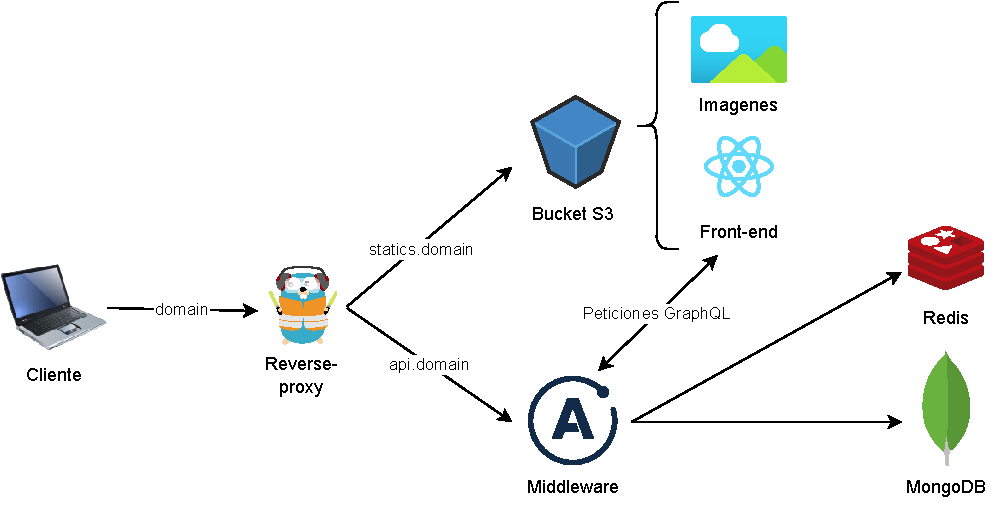
\includegraphics{../drawio/general.drawio-1.pdf}
		}
		\caption{Diseño original a alto nivel (O. Salvador, 2022)}
	\end{figure}

Las necesidades de las piezas principales de la aplicación han dictado la infraestructura que he implementado, iterando sobre el. Con la correcta configuración de CORS en el almacenamiento de \textit{Blobs} es posible mantener la seguridad sin necesitar un proxy inverso. Cabe resaltar que en mi modelo actual todos los componentes están expuestos a internet, teniendo todos una dirección IP, y el front-end un FQDN.
\linebreak

	\begin{figure}[htb]
		\centering
		\resizebox{.8\linewidth}{!}{%
			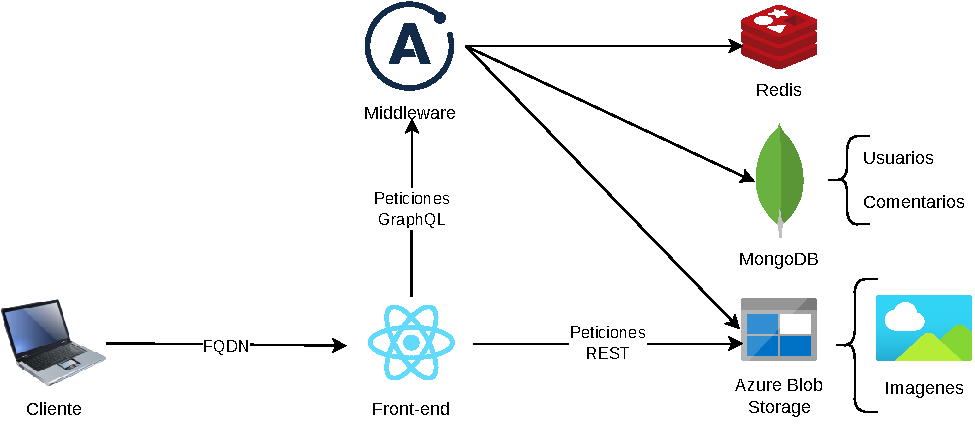
\includegraphics{../drawio/general2.drawio.pdf}
		}
		\caption{Diseño revisado (O. Salvador, 2022)}
		\label{alto_nivel}
	\end{figure}


	\subsection{Acceso a la página}
	He escrito el front-end en TypeScript, lo que hace necesario compilar los fuentes (\texttt{.tsx}) a JavaScript. Entrare en detalle sobre como son servidos estos y el resto de estáticos del frontal en la sección dedicada a infraestructura. 
	\linebreak
	
	El usuario accede al servidor del frontal y baja los archivos de la página a su navegador. Desde ahi, el cliente hace peticiones GraphQL al backend y REST al \textit{Azure Blob Storage}. La primera petición que hace el cliente es al backend, recuperando la lista de \textit{posts}. Para hacerlo, el backend usa un \textit{connection string} para enlazar con la base de datos Mongo. En esta petición no es necesario que el usuario este autenticado, no tendría sentido pedirle los credenciales tan pronto. 
	\linebreak
	
	La lista de \textit{posts} contiene la direcciones de la imágen y autor de cada uno. He configurado el almacen para permitir lectura publica. El cliente renderiza cada comentario, recuperando una a una las imagenes, y, si el usuario estuviese autenticado, mostrandole la opción de borrar aquellos de los que sea autor.
	\linebreak
	
	
		\begin{figure}[htb]
			\centering
			\resizebox{.9\linewidth}{!}{%
				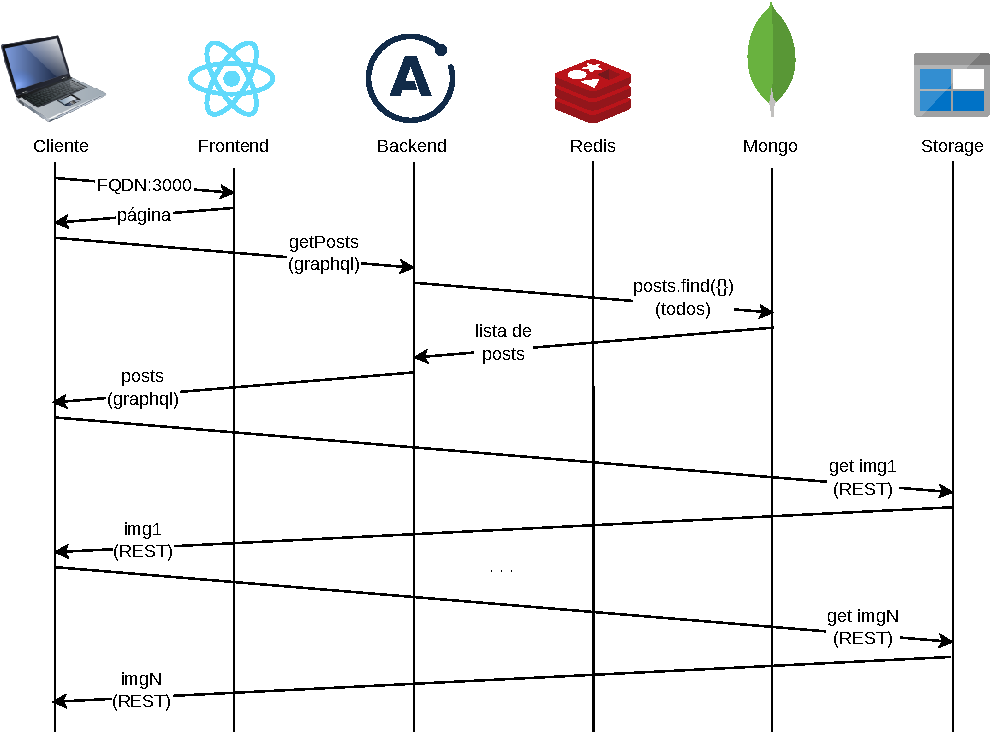
\includegraphics{../drawio/getposts.drawio.pdf}
			}
			\caption{Paso de mensajes \texttt{getPosts()} (O. Salvador, 2022)}
		\end{figure}
	
	\bigskip
	\bigskip
		
	\subsection{Registro e inicio de sesión}
	Con la pagina renderizada el usuario puede ver una opción en la esquina superior derecha, ``Login''. Hacer click sobre el botón despliega un \textit{modal}, un desplegable de React. 
	\linebreak
	
	Dentro de este se le piden nombre de usuario y contraseña. La primera vez que entre, no tendrá cuenta y deberá registrarse. En el modal hay dos solapas, ``Login'' y ``Register''. Elegir la segunda cambiara el modal por uno dedicado al registro. Este comparte los campos del anterior, y añade una segunda entrada para confirmar la contraseña. En el cliente se comprueba la contraseña: los valores de los campos de contraseñas tienen que ser iguales, una contraseña debe tener al menos cuatro caracteres, una  minúscula, mayúscula, número, y carácter especial. Si valen, se envía una petición al backend para guardar el usuario. Este comprueba en Mongo si ya existe uno con ese nombre, de hacerlo niega la creación. En caso contrario, se crea.
	\linebreak
	
		\begin{figure}[htb]
			\centering
			\begin{subfigure}{.9\textwidth}
				\hspace{-3cm}
				\inputminted[fontsize=\scriptsize, firstline=74, lastline=74, linenos, frame=single, tabsize=1]{javascript}{../../frontend/src/components/LoginPrompt.tsx}
				\caption{Verificación de carácteres de la contraseña, frontend, \texttt{LoginPrompt.tsx} (O. Salvador, 2022)}
			\end{subfigure}
			\linebreak
			
			
			
			\begin{subfigure}{.9\textwidth}
				\hspace{-3cm}
				\inputminted[fontsize=\scriptsize, firstline=153, lastline=160, linenos, frame=single]{javascript}{../../backend/src/resolvers/mutation.js}
				\caption{Comprobación del usuario contra la base de datos, backend, \texttt{mutation.js} (O. Salvador, 2022)}
			\end{subfigure}
			

			\caption{Proceso de registro, (O. Salvador, 2022)}
		\end{figure}
		
	La operación de registro desata un inicio de sesión automáticamente al acabar. En esta, al buscar en la base de datos, con usuario y contraseña, si no hay una entrada en la que ambas encajen con la petición, se responde con error. El error es genérico, ``User or password incorrect'', deliberadamente no confirmando si existe el usuario, por seguridad. 
	\linebreak
	
	De ser un éxito, el backend a continuación genera una cadena de caracteres aleatoria y guarda este token, junto con su usuario, en la base de datos Redis. He diseñado la función de manera que los tokens caduquen automáticamente después de una hora, y se eliminen del Redis. Como he planteado el sistema, un mismo usuario puede tener varias sesiones abiertas a la vez. Al responder al cliente le pasa este token, que a continuación se guarda como cookie en el navegador.
	\linebreak
	
		\begin{figure}[htb]
			\centering
			\resizebox{.5\linewidth}{!}{%
				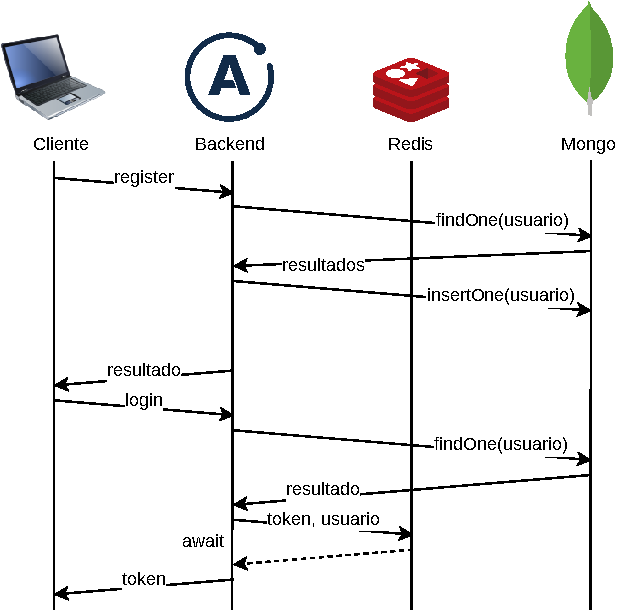
\includegraphics{../drawio/register.drawio.pdf}
			}
			\caption{Peticiones \texttt{register()} y consecuente \texttt{login()} (O. Salvador, 2022)}
		\end{figure}
	
	En la entrega parcial tenía como objetivo tunelizar el trafico del cliente al backend. Al pasar el trafico por TLS, no sería necesario cifrarlo en la propia aplicación. No he sido capaz de implementar los certificados necesarios para que la conexión sea \texttt{https}. Como resultado, los credenciales son interceptables
	\linebreak
	
	\begin{figure}[htb]
		\centering
		\resizebox{.95\linewidth}{!}{%
			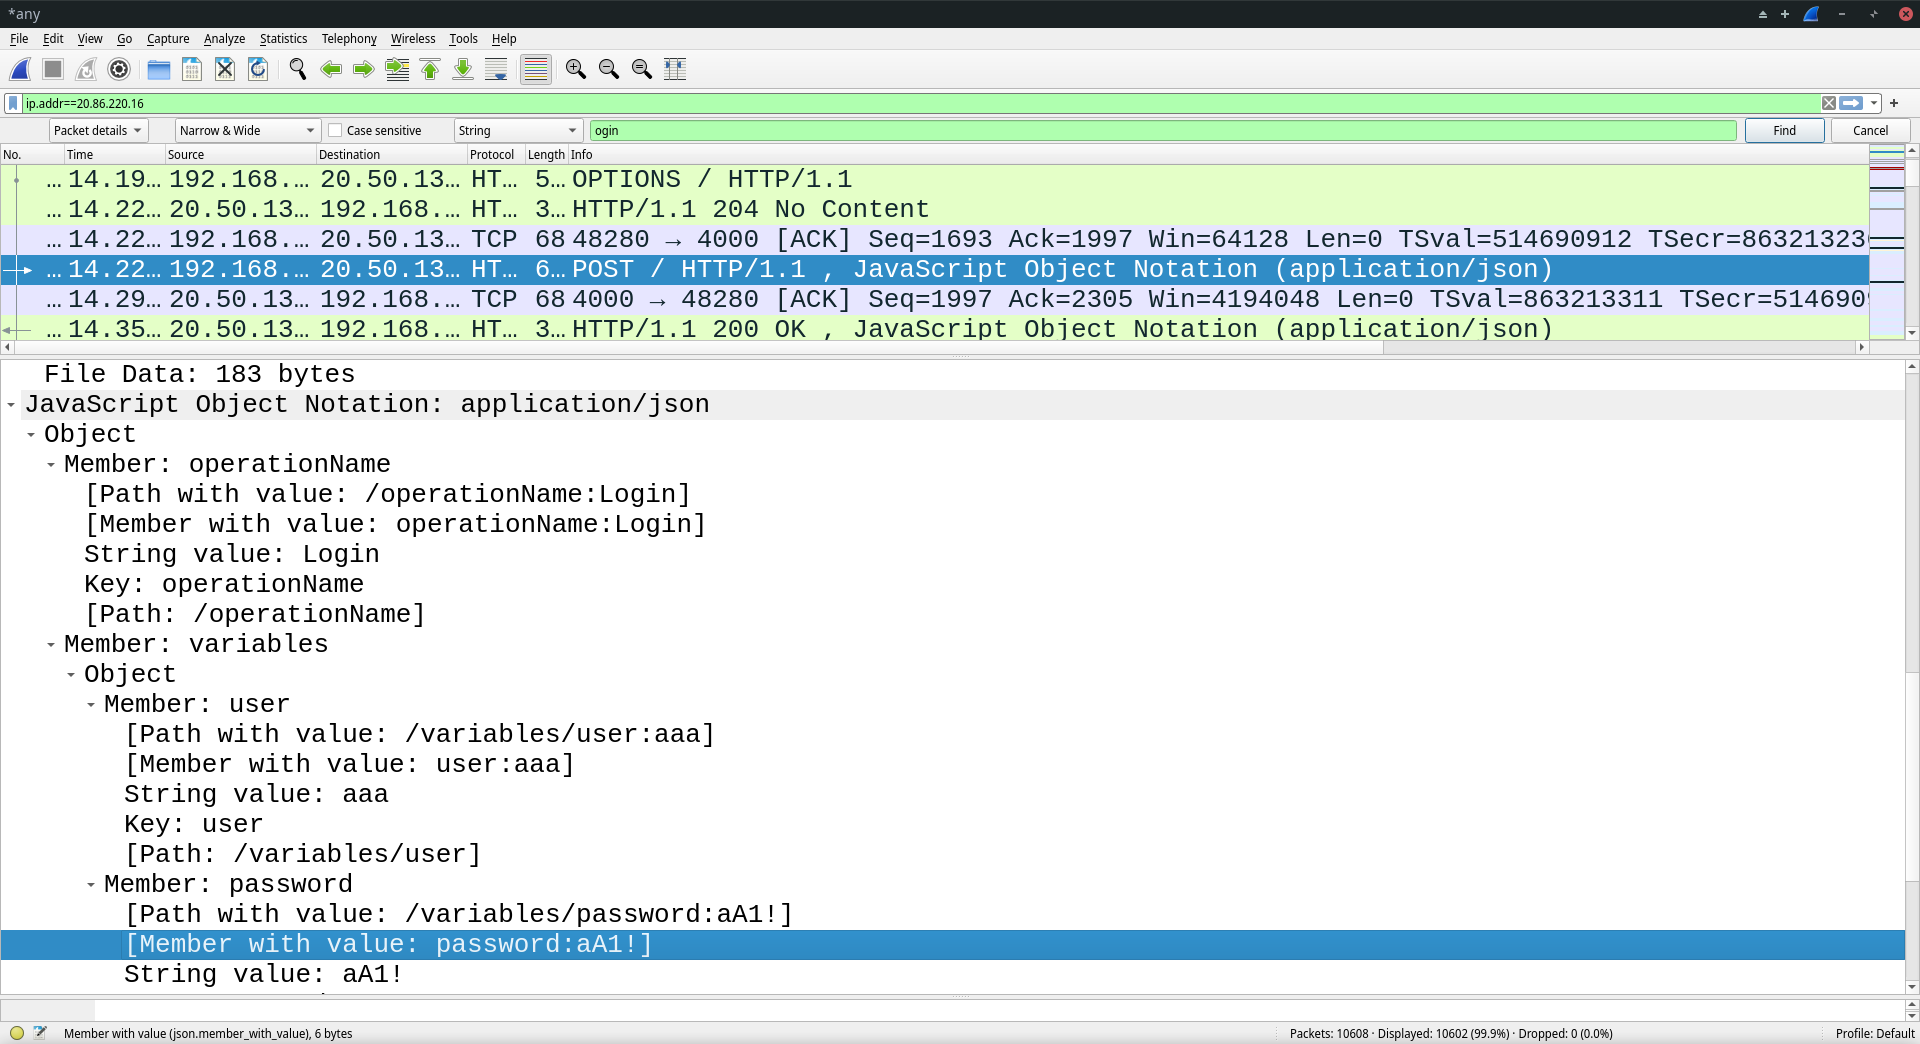
\includegraphics{../capturas/azure_wireshark_password.png}
		}
		\caption{Cabeceras en la petición del navegador (O. Salvador, 2022)}
	\end{figure}
	
	Todas las demás peticiones requieren que el usuario esté autenticado. En todas se espera que la petición venga con un token, y en cada una de ellas se comprueba este contra la base de datos Redis. Creo un único cliente de Redis para el backend, y lo uso para resolver el token a un usuario. Paso el usuario y cliente a cada función por el contexto de ejecución de ApolloServer. Las funciones que necesitan verificación comprueban el usuario. Algunas que necesitan conectarse a Redis ahorran crear su propio cliente. Durante la integración de Redis en el backend usé el siguiente articulo de Humberto Leal \cite{rediscode}.
	\linebreak
	
		\begin{figure}[htb]
			\centering

			\begin{subfigure}{.4\textwidth}
				\inputminted[fontsize=\scriptsize, firstline=17, lastline=24, frame=single, breaklines]{javascript}{../../backend/src/index.js}
				\caption{Declaración, \texttt{index.js}}
			\end{subfigure}
			\hspace{1cm}
			\begin{subfigure}{.5\linewidth}
				\inputminted[fontsize=\scriptsize, firstline=53, lastline=53, frame=single, breaklines]{javascript}{../../backend/src/index.js}
				\vspace{-.6cm}
				\inputminted[fontsize=\scriptsize, firstline=65, lastline=65, frame=single, breaklines, gobble=3]{javascript}{../../backend/src/index.js}
				\vspace{-.6cm}
				\inputminted[fontsize=\scriptsize, firstline=71, lastline=71, frame=single, breaklines, gobble=3]{javascript}{../../backend/src/index.js}
				\vspace{-.6cm}
				\inputminted[fontsize=\scriptsize, firstline=84, lastline=84, frame=single, breaklines, gobble=3]{javascript}{../../backend/src/index.js}
				\vspace{.55cm}
				\caption{Conexión y paso por contexto, \texttt{index.js}}
			\end{subfigure}
			\linebreak
			
			\begin{subfigure}{.6\textwidth}
				\inputminted[fontsize=\scriptsize, firstline=57, lastline=61, linenos, frame=single, breaklines]{javascript}{../../backend/src/resolvers/mutation.js}
				\caption{Uso del nombre de usuario resuelto para autorizar \texttt{mutation.js}}
			\end{subfigure}
			
			\caption{Extractos de código del backend para trabajar con Redis (O. Salvador, 2022)}
			\label{extractos_redis}
		\end{figure}
  
  \bigskip
  \bigskip
  
	\subsection{Creación de ``\textit{Posts}''}
	Una vez el usuario se ha identificado, el botón ``Login'' queda sustituido por dos: ``Post'' y ``Logout''. Al pulsar el primero, aparecerá un nuevo modal. En el hay dos botones a su vez, uno al que se puede arrastrar una imagen para adjuntarla al comentario, y otro para quitarla, para que el usuario pueda cambiar de elección. Al elegir una imagen, se muestra en el modal una vista previa de ella.  Para conseguir esta funcionalidad he usado un paquete de \textit{npm} separado, \textit{react-images-uploading} (\cite{react_imgs}). Mi implementación se basa en su código de referencia, pero considerablemente editado, ya que mi uso es mas limitado que el que demuestran en el.
	\linebreak
	
	En el modal hay un campo de texto, para escribir un comentario que acompañe a la imagen. Al escribir algo sobre este, aparecerá un botón a su derecha para subir el \textit{post}. Cuando el backend recibe la petición \texttt{addPost()} del cliente, no recibe ninguna imagen, solo el autor y el comentario. Después de autenticarlo, genera una \textit{URL pre-firmada}. Sube esta y el comentario del \textit{post}, junto con el autor a Mongo. Por último, devuelve la URL al frontend, que se conecta al almacen y sube la imagen directamente.
	\linebreak
	
	El almacen tiene restricciones de acceso, por seguridad. Permite leer sus contenidos libremente, pero solo alguien autorizado puede subir nuevos. Pasar los credenciales de administración del almacén al frontend presenta un riesgo de seguridad. Hacerlo en el backend, donde podrían estar con menos riesgo, presenta dos: además del desafío que es subir la imagen a Azure, subirla al backend primero; y el trafico añadido, ya que ahora el backend tiene primero que bajarse la imagen y luego subirla. Mitigo completamente el problema de seguridad no dándole al frontend mas que lo mínimo para que suba la imagen. Este mínimo es la URL pre-firmada.
	\linebreak
	
	Aunque el término viene de la implementación de AWS, en Azure se puede conseguir un resultado similar. Primero importo del entorno de ejecución del proceso las variables con los credenciales de administración del almacén, aquí no son preocupantes. Con ellas genero una llave de acceso compartido \textit{StorageSharedKeyCredential} y con esta una firma de acceso compartido. Uso esta para generar una URL en la que se puede crear un Blob. Tiene una caducidad de una hora y solo permite crear uno. Esta llave desechable va embebida en la URL, que devuelvo como respuesta a la petición. Esta ha sido una de las partes más complicadas, y he usado extensivamente la documentación de Mirosoft, en particular: \cite{ms_add_blob1}, \cite{ms_add_blob2}, \cite{ms_add_blob3}, \cite{ms_add_blob4}, y \cite{ms_add_blob5}.
	\linebreak
	
		\begin{figure}[htb]
			\centering
			\begin{subfigure}{0.41\textwidth}
				\inputminted[fontsize=\scriptsize, firstline=24, lastline=27, frame=single, breaklines, gobble=7]{javascript}{../../backend/src/resolvers/mutation.js}
				\vspace{.45cm}
				\caption{Credenciales, cuenta de almacenamiento}
			\end{subfigure}
			\hspace{1cm}
			\begin{subfigure}{0.5\textwidth}
				\inputminted[fontsize=\scriptsize, firstline=34, lastline=38, frame=single, breaklines, gobble=7]{javascript}{../../backend/src/resolvers/mutation.js}
				\caption{Creación de la \textit{Shared Access Signature}}
			\end{subfigure}
						
			\caption{Uso de credenciales de almacenamiento, backend, \texttt{mutation.js} (O. Salvador, 2022)}
		\end{figure}
		
	De vuelta en el frontend, subir la imagen es una simple petición REST, usando \texttt{fetch()} para hacer un \texttt{PUT} de la imagen que el usuario ha subido al cliente a ella.

	
	
	\clearpage
	\subsection{Eliminación de ``\textit{Posts}''}
	Cuando el usuario (autenticado) tenga uno o mas \textit{posts} a su nombre, al renderizar la página, el cliente los marcará con la opción de eliminarlos. Si el usuario hace click sobre esta opción, el cliente alimentará el identificador del \textit{post} a la función \texttt{removePost()} 
	\linebreak
	
	En el backend, se comprueba si el token del cliente es válido, y si el identificador de \textit{post} representa uno existente. Superadas estas dos condiciones, se comprueba que el nombre del usuario es el mismo que el del autor. Es importante recalcar que esta comprobación no depende solo de la implementación del frontend, se hace dos veces. Antes de borrar la entrada en la base de datos, borro la imagen del almacen. Aunque me costó más aprender a subir las imágenes, borrarlas también ha sido dificil. El articulo que mas me ha ayudado ha sido \cite{ms_rm_blob}, igual que los otros, de la documentación de Microsoft.
	\linebreak
	
	Igual que en la creación, recupero los credenciales para acceder al almacén de las variables de entorno y la junto en una \textit{StorageSharedKeyCredential}. Con esta creo un cliente para el contenedor, y con este, un cliente para el blob de la imagen elegida. Si la imagen existe, la borro. Después del borrado, elimino su entrada en la base de datos Mongo.
	\linebreak
	
	\begin{figure}[htb]
			\centering
			\begin{subfigure}{0.9\textwidth}
			\inputminted[fontsize=\scriptsize, firstline=104, lastline=104, linenos, frame=single, breaklines]{javascript}{../../backend/src/resolvers/mutation.js}
			\vspace{-.6cm}
			\inputminted[fontsize=\scriptsize, firstline=107, lastline=110, linenos, frame=single, breaklines]{javascript}{../../backend/src/resolvers/mutation.js}
			\vspace{-.6cm}
			\inputminted[fontsize=\scriptsize, firstline=118, lastline=118, linenos, frame=single, breaklines]{javascript}{../../backend/src/resolvers/mutation.js}
			\vspace{-.6cm}
			\inputminted[fontsize=\scriptsize, firstline=126, lastline=126, linenos, frame=single, breaklines]{javascript}{../../backend/src/resolvers/mutation.js}
			\end{subfigure}
			\caption{Comando de arranque del servidor, \texttt{Dockerfile} (O. Salvador, 2022)}
		\end{figure}

	\bigskip
	\bigskip
	
	\subsection{Cierre de sesión}
	Esta operación es muy corta, el cliente manda una petición al backend para que este borre la entrada de la base de datos Redis. Al recibir la respuesta confirmando la eliminación, borra la cookie del navegador del usuario.
	\linebreak













\clearpage
\section{Infraestructura e integración}
Uso una mezcla heterogénea de servicios de Azure para satisfacer las necesidades de los componentes mencionados a alto nivel en la Figura \ref{alto_nivel} (p. \pageref{alto_nivel}), dejando atrás la simplicidad de la primera fase de entrega, donde todos los componentes eran contenedores manejados con Docker Compose. Los componentes necesarios para que el sistema funcione son:
	\begin{enumerate}
		%\addtolength{\itemindent}{0.80cm}
		\itemsep0em 
		\item \textbf{Grupo de recursos} con el que contener a todos los demás, y mantenerlos organizados.
		\item \textbf{Red virtual} para poder acceder a los recursos que quiero públicos. Algunos, como los grupos de contenedores lo necesitan.
		\item \textbf{Cuenta de almacenamiento} y \textbf{contenedor de almacenamiento} donde hospedar las imágenes con contenedores de ``blobs''.
		\item \textbf{Registro de contenedores} al que subir las imagenes del frontend y backend.
		\item \textbf{CosmoDB}, la solución de base de datos de Azure, con compatibilidad para MongoDB.
		\item \textbf{Redis} como cache para los tokens.
		\item \textbf{Instancias de contenedores}, una de las soluciones de Azure para correr contenedores.
	\end{enumerate}

	\begin{figure}[htb]
		\centering
		\resizebox{.85\linewidth}{!}{%
			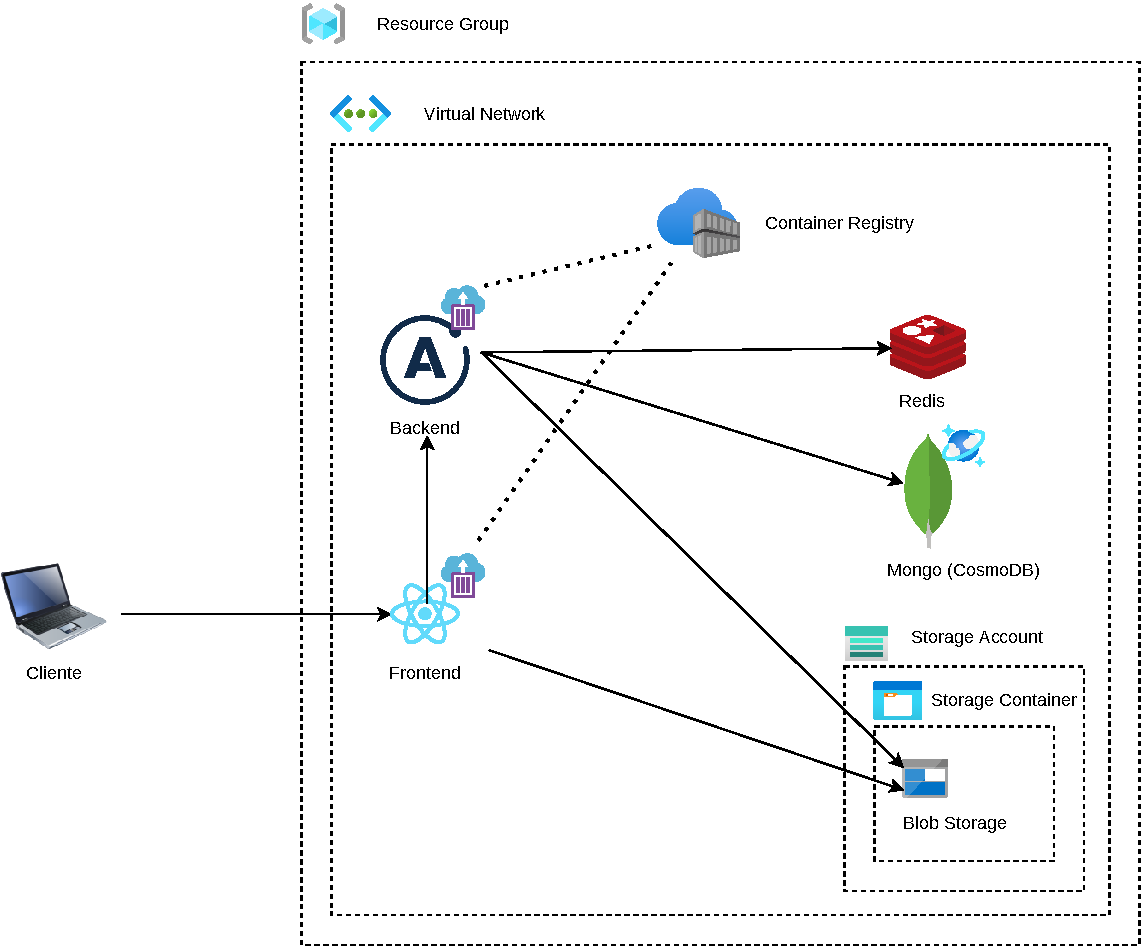
\includegraphics{../drawio/general-infra.drawio.pdf}
		}
		\caption{Diagrama de infraestructura (O. Salvador, 2022)}
	\end{figure}





	\clearpage
	\subsection{Bases de datos}
	El sistema necesita dos BBDD: una documental para almacenar los \textit{posts} y usuarios de forma persistente; y una llave-valor para almacenar impermanentemente las parejas token-usuario. Originalmente diseñe el sistema en local, con ambas suplidas por contenedores, con las imagenes oficiales \texttt{mongo:latest} y \texttt{redis/redis-stack:latest}. Las dos permiten su uso en local, para desarrollo, sin autenticación. Este no es el caso en producción, en Azure ambas necesitan credenciales para poder acceder, detallare la implementación de estos en la siguiente sección.
	\linebreak
	
	Desde el 16 de Octubre, 2018, MongoDB Inc. ha publicado las nuevas versiones de su software bajo la licencia SSPL (\textit{Server Side Public Licence}) (\cite{mongo_sspl}). Esta es una licencia de código libre, que permite la copia y distribución, basada en AGPLv3, pero con el requisito añadido de que cualquier proveedor cloud que ofrezca la funcionalidad del software con esta licencia debe publicar la enteridad de \underline{su} código fuente. Esto incluye software, APIs y cualquier otro componente necesario para replicar la solución del proveedor. 
	\linebreak
	
	Como resultado de este cambio, plataformas cloud como la ofrecida por Microsoft pasaron a ofrecer alternativas compatibles con MongoDB, pero resultado de un desarrollo independiente. En el caso de Azure, su solución de base de datos es CosmoDB, y tiene un modo de uso compatible con aplicaciones diseñadas para Mongo. 
	\linebreak
	
	En mi experiencia durante este proyecto, los desarrolladores de esta alternativa han conseguido un éxito completo. La integración de mi aplicación con esta solución fue admirablemente trivial. Solo tuve que cambiar la URL de mi cliente por un \textit{Connection String} a la nueva. En esta cadena de caracteres van incluidos los credenciales. El backend la recibe como variable de entorno, por lo que no tuve siquiera que tocar su código.
	\linebreak
	
		\begin{figure}[htb]
			\centering
			\hspace{.5cm}
			\begin{subfigure}{0.4\textwidth}
				\inputminted[fontsize=\scriptsize, firstline=47, lastline=47, linenos, frame=single, breaklines]{javascript}{../../backend/src/index.js}
				\vspace{-.6cm}
				\inputminted[fontsize=\scriptsize, firstline=54, lastline=54, linenos, frame=single, breaklines]{javascript}{../../backend/src/index.js}
				\vspace{-.6cm}
				\inputminted[fontsize=\scriptsize, firstline=67, lastline=67, linenos, frame=single, breaklines, gobble=6]{javascript}{../../backend/src/index.js}
				\vspace{-.6cm}
				\inputminted[fontsize=\scriptsize, firstline=84, lastline=84, linenos, frame=single, breaklines, gobble=6]{javascript}{../../backend/src/index.js}
				\caption{\texttt{index.js}}	
			\end{subfigure}
			\hspace{1.3cm}
			\begin{subfigure}{0.45\textwidth}
				\inputminted[fontsize=\scriptsize, firstline=57, lastline=57, linenos, frame=single, breaklines, gobble=3]{javascript}{../../backend/src/resolvers/mutation.js}
				\vspace{-.6cm}
				\inputminted[fontsize=\scriptsize, firstline=59, lastline=59, linenos, frame=single, breaklines, gobble=5]{javascript}{../../backend/src/resolvers/mutation.js}
				\vspace{-.6cm}
				\inputminted[fontsize=\scriptsize, firstline=68, lastline=68, linenos, frame=single, breaklines, gobble=7]{javascript}{../../backend/src/resolvers/mutation.js}
				\caption{\texttt{mutation.js}}	
			\end{subfigure}
			\caption{Ejemplo de uso de MongoDB en el backend (O. Salvador, 2022)}
		\end{figure}
		
	Por su parte, integrar Redis también fue sencillo. Además de alimentarle la URL en la que encontrar al servidor he tenido que darle el puerto y contraseña, especificando en el cliente que es trafico tunelizado, ver Figura \ref{extractos_redis} (p. \pageref{extractos_redis}).
	\linebreak
	
	Azure ofrece interfaces a ambos, para poder depurar. En el caso de CosmosDB, un interfaz gráfico, \textit{Data Explorer} con el que conseguir la misma funcionalidad que satifací durante el desarrollo en local con el interfaz provisto por Mongo en la imagen \texttt{mongo-express:latest}.
	\linebreak
			
		\begin{figure}[htb]
			\centering
			\resizebox{\linewidth}{!}{%
				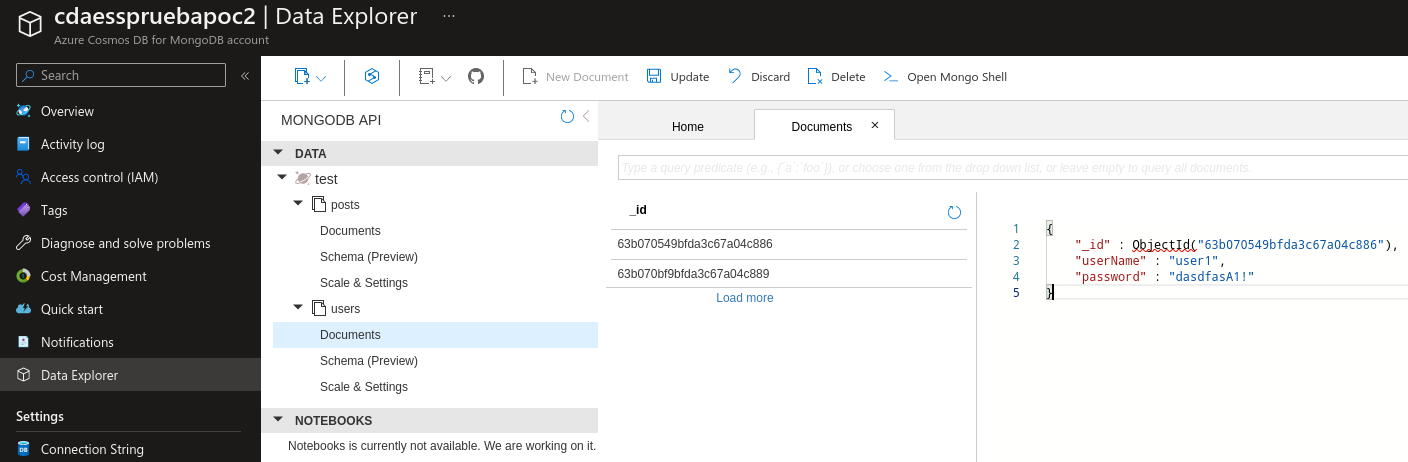
\includegraphics{../capturas/azure_cosmo_data_explorer.png}
			}
			\caption{Azure Data Explorer, colección ``users'' (O. Salvador, 2022)}
		\end{figure}
		
	En el caso de Redis es una linea de comandos, accesible desde el portal de Azure, dentro del recurso, con la opción ``Console''. Comandos como ``\texttt{keys *}'' para poder ver todas las llaves que tiene guardadas en ese momento. 
	\linebreak
	
		\begin{figure}[htb]
			\centering
			\resizebox{.8\linewidth}{!}{%
				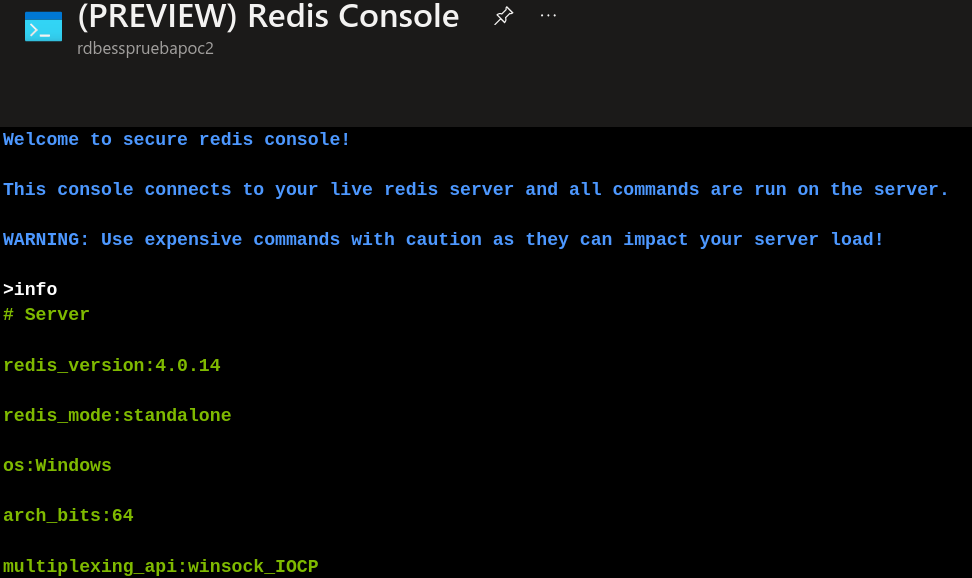
\includegraphics{../capturas/azure_redis_windows.png}
			}
			\caption{Consola de Redis desde el portal de Azure (O. Salvador, 2022)}
			\label{consola_redis}
		\end{figure}
	
	
	\clearpage
	A diferencia de los otros componentes, como el frontend, backend, o almacenamiento de blobs, tanto Mongo como Redis usan su propio protocolo. Esto implica que para poder acceder al servicio desde fuera del portal de Azure es necesario tener un cliente adecuado. En el caso de Redis, la misma imagen \texttt{redis/redis-stack:latest} incluye \texttt{redis-cli}, un cliente de Redis por linea de comandos. Cabe resaltar que en la siguiente imagen me conecté de manera insegura (puerto 6379), después de manualmente editar la configuración que despliego como código, en la que solo permito conexiones tunelizadas (puerto 6380). Es posible establecer un tunel y conectarse de manera segura, \cite{redis_connect}, aún si no lo he hecho para esta práctica.
	\linebreak
	
		\begin{figure}[htb]
			\centering
			\resizebox{\linewidth}{!}{%
				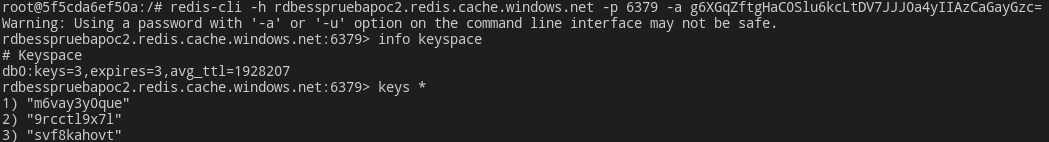
\includegraphics{../capturas/azure_redis-cli.png}
			}
			\caption{Listado de llaves con \texttt{redis-cli} en contenedor (O. Salvador, 2022)}
		\end{figure}
	
	Las bases de datos son los elementos mas pesados de levantar, pero curiosamente Redis tarda mas que CosmoDB. Mi explicación para este fenómeno es que CosmosDB este diseñado completamente por el equipo de Microsoft, mientras que Redis se levante como aplicación de terceros en el contenedor o maquina virtual que utilicen. Aparte del motor de virutalización que usen, como se ve en la Figura \ref{consola_redis}, corre sobre Windows, que siempre es más pesado que sus alternativas basadas en Linux. Como el código es cerrado, esto es solo especulación. En la todas las ejecuciones de \texttt{terraform apply} en las que despliego Redis, es el componente que más tarda, casi siempre superando los veinte minutos.
	\linebreak
	
	\begin{figure}[htb]
		\centering
		\resizebox{.6\linewidth}{!}{%
			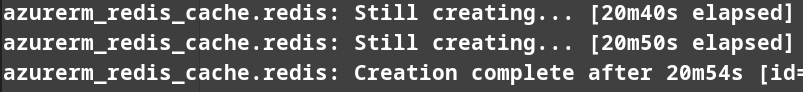
\includegraphics{../capturas/azure_redis_20min.png}
		}
		\caption{Tiempo necesario para aprovisionar Redis usando Terraform (O. Salvador, 2022)}
	\end{figure}

	
	\bigskip
	\bigskip
	
	\subsection{Grupos de contenedores}
	Azure ofrece varias soluciones para hospedar aplicaciones web según el nivel de control que el cliente desee sobre la infraestructura. Sus soluciones relevantes principales son: Azure Kubernetes Service (AKS), Azure Container Instance (ACI) y Azure Container Apps (APA). La primera ofrece control completo sobre el clúster en el que se ejecutan los contenedores, junto con el trabajo que implica manejarlos manualmente. La última abstrae demasiado y dificulta parte de la gestión que quería realizar. Como resultado, he elegido utilizar grupos de contenedores, ACI para los servidores de tanto el frontend como el backend.
	\linebreak
	
	Para poder levantar una instancia de contenedor, Azure necesita tener su imagen disponible. Se pueden elegir imagenes de \texttt{hub.docker.com}, pero he preferido crear mi propio registro dentro del proyecto y subir ahi mis imagenes. Subirlas sigue el mismo proceso que a cualquier otro registro, después de hacer login en \texttt{azure-cli} es necesario hacerlo en el registro particular, y luego empujar la imagen.
	\linebreak
	
	\begin{figure}[htb]
		\centering
		\begin{subfigure}{.9\linewidth}
		\scriptsize
		\texttt{\$ az acr login -n <NOMBRE\_DE\_REGISTRO>} 
				
		\texttt{\$ docker build -t fullstackpoc-front:1.0.0 .}
		
		\texttt{\$ docker tag fullstackpoc-front:1.0.0 <NOMBRE\_DE\_REGISTRO>.azurecr.io/fullstackpoc-front:latest} 
		
		\texttt{\$ docker push <NOMBRE\_DE\_REGISTRO>.azurecr.io/fullstackpoc-front:latest} 
		\end{subfigure}
		
		Comandos para subir la imágen del frontend
	\end{figure}

	He tenido problemas para conseguir generar las imágenes, el desarrollo en local donde ambos son contenedores no es representativo de conseguir \textit{dockerizar} las aplicaciones y prepararlas para un entorno de producción. El backend, escrito en JavaScript fue sencillo, solo necesitando una instalación de los paquetes que uso antes de poder servir los contenidos del proyecto. Por el contrario, el frontend, escrito en TypeScript fue más complicado. A parte de las dependencias de Node son necesarias las demandadas por React y compilar el proyecto a JavaScript. Además, no se pueden servir de la misma manera, necesita un servidor específico. Antes de usar el paquete \textit{serve} de Node usaba una imagen de Nginx\footnote{El \texttt{Dockefile} en el que compilaba el proyecto con una imagen de Node y luego pasaba \texttt{/build} a una segunda imagen, de Nginx para servirla está disponible en la carpeta del frontend, ``Dockerfile-nginx''. Me base en: \cite{docker_nginx1}, \cite{docker_nginxi2} y \cite{docker_nginx3}}. Pero en ambos la página era estática, no ejecutando las peticiones GraphQL. He conseguido solucionarlo como muestro en el extracto. Compilo el proyecto inmediatamente antes de servirlo. Tropecé con esta solución por mi cuenta. No he podido responder el por que así si funciona.
	\linebreak
	
		\begin{figure}[htb]
			\centering
			\begin{subfigure}{0.3\textwidth}
				\inputminted[fontsize=\scriptsize, firstline=21, lastline=22, linenos, frame=single, breaklines]{dockerfile}{../../backend/Dockerfile}
			\caption{\texttt{Dockerfile} del backend}
			\end{subfigure}
			\hspace{1.5cm}
			\begin{subfigure}{0.5\textwidth}
				\inputminted[fontsize=\scriptsize, firstline=36, lastline=37, linenos, frame=single, breaklines]{dockerfile}{../../frontend/Dockerfile}
			\caption{\texttt{Dockerfile} del frontend}
			\end{subfigure}

			\caption{Comandos de arranque de los servidores contenedorizados (O. Salvador, 2022)}
		\end{figure}

	\clearpage
	Docker esta orientado a capas. En mi opinión, su sistema de ficheros (AuFS) orientado a capas es su valor principal, por encima del uso directo del kernel del huesped, frente a las máquinas virtuales tradicionales. En mis \texttt{Dockefile} uso generosamente las instrucciones ``\texttt{RUN}'' y ``\texttt{COPY}'', cadad una de ellas generando una nueva capa. Antiguamente tantas capas habrían reducido el rendimiento por sobre-abstracción, pero en las nuevas versiones no tiene tanto efecto, ya que se compactan (\cite{docker_layers}), y mis imagines son pequeñas. El beneficio de generar varias capas es evidente en la construcción de las imágenes y en su subida al registro (ACR). Docker comparte las capas entre imágenes. Esto implica que durante la depuración, puede solo ser necesario instalar las dependencias de un proyecto una vez, todas las imágenes que compartan esa capa partiendo de su progreso. Tambien significa que solo es necesario subir las capas que sean distintas de las que el registro ya tiene, como muestro en la figura, subiendo la imágen del frontend después de haber subido el backend.
	\linebreak
	
	\begin{figure}[htb]
		\centering
		\resizebox{.7\linewidth}{!}{%
			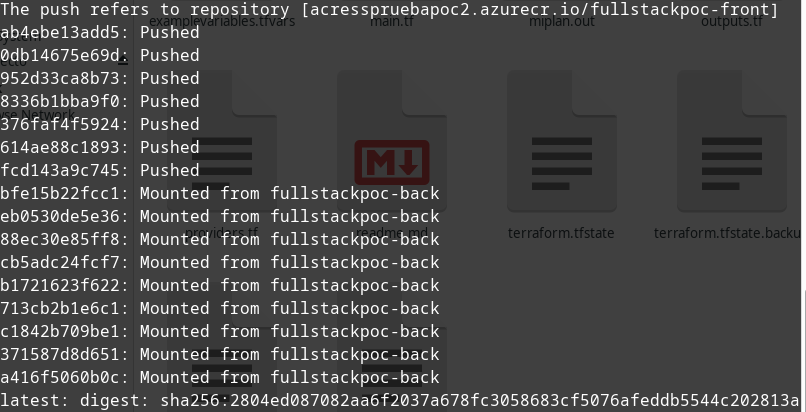
\includegraphics{../capturas/azure_acr_reutiliza_capas_entre_contenedores.png}
		}
		\caption{Azure Container Registry compartiendo capas entre imágenes (O. Salvador, 2022)}
	\end{figure}
	
	Con las imágenes disponibles, Azure puede empezar a desplegar los grupos de contenedores. Por dependencias entre los componentes, es necesario construir la infraestructura en pasos. Primero el grupo de recursos, red virtual, bases de datos, y almacenamiento de blobs; Segundo el backend; Y tercero el frontend. No se pueden exportar variables en el Dockerfile, Azure no las sobreescribe.
	\linebreak
	
	El backend necesita tener acceso a las bases de datos y almacenamiento, al arrancar lo primero que hace es intentar montar un cliente con Redis y otro con Mongo. Si no tiene sus direcciones y credenciales como variables de entorno al arrancar, fracasara su ejecución, y Azure reiniciara el contenedor. Esto pasará en bucle. El frontend tiene la misma dependencia con el backend, e implícitamente con los demás componentes a través de el. En la siguiente figura muestro, simbólicamente, las direcciones de los componentes, y como se conectan entre sí, además del orden en el que hay que aprovisionarlos.
	\linebreak	
				
		\begin{figure}[htb]
			\centering
			\resizebox{.7\linewidth}{!}{%
				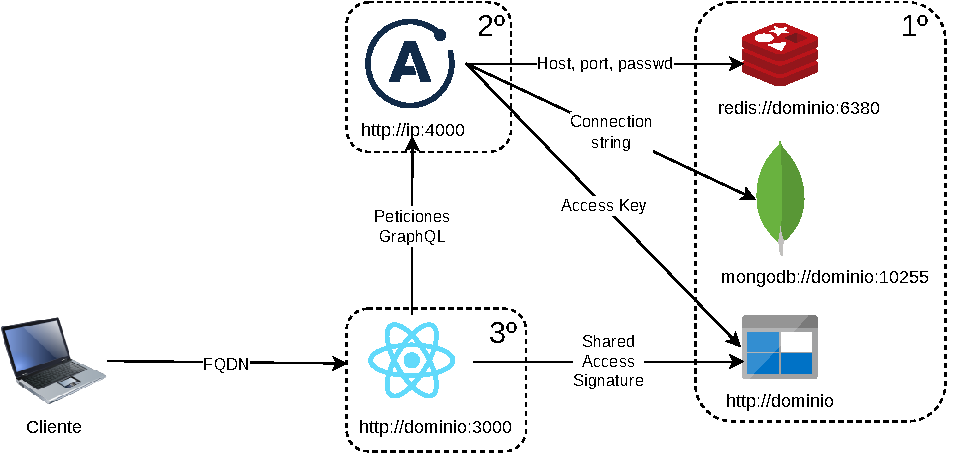
\includegraphics{../drawio/general2-resueltos.drawio.pdf}
			}
			\caption{Diagrama a alto nivel, conexiones y orden de aprovisionado (O. Salvador, 2022)}
		\end{figure}		
		
	Durante el desarrollo, ApolloServer, la librería que uso para el servidor de GraphQL en el backend, publica un interfaz gráfico desde el que hacer peticiones para la depuración. Por defecto este se deshabilita en producción. Se puede especificar que siga disponible, pero es mala praxis mantenerlo cuando la aplicación está publicada. Para poder seguir depurando en producción, he vuelto a usar cURL. GraphQL sigue siendo REST aunque parezca una tecnología distinta a primera vista. A continuación dos ejemplos de peticiones al backend: \texttt{getPosts()} (solo había un \textit{post}) y \texttt{login()}, con el usuario con el que me identifico en el Data Explorer de CosmosDB de fondo.
	\linebreak
	
		\begin{figure}[htb]
			\centering
			\begin{subfigure}{\textwidth}
				\resizebox{\linewidth}{!}{%
					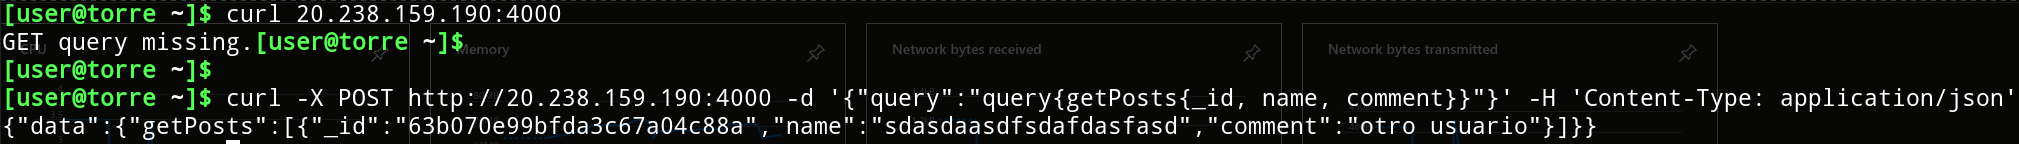
\includegraphics{../capturas/azure_depuracion_curl.png}
				}
				\footnotesize
				\texttt{\$ curl -v -X POST http://<IP>:4000 -d '\{"query":"query\{getPosts\{\_id, name, comment\}\}"\}' -H 'Content-Type: application/json'} 
				\caption{Petición \texttt{getPosts()}}
			\end{subfigure}
			\linebreak
			
			\begin{subfigure}{\textwidth}
				\begin{subfigure}{\textwidth}
				\centering
				\resizebox{.7\linewidth}{!}{%
					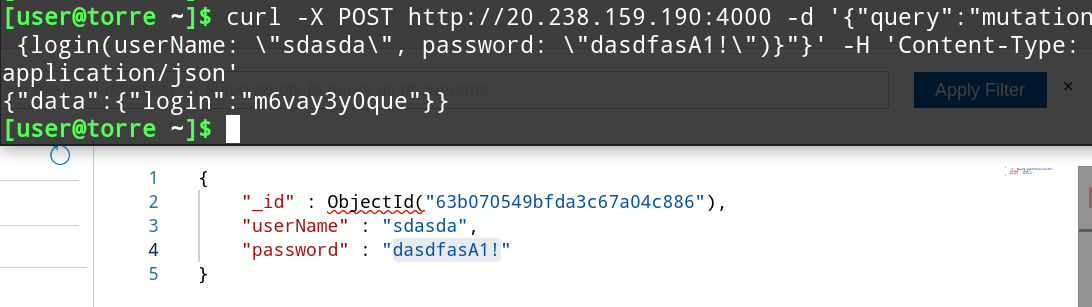
\includegraphics{../capturas/azure_login_curl_explorer_fondo.png}
				}
				\end{subfigure}
				\linebreak
				\footnotesize
				\texttt{\$ curl -v -X POST http://<IP>:4000 -d '\{"query":"mutation \{login(userName: \textbackslash"\ <USERNAME>\ \textbackslash"\ , password: \textbackslash"\ <PASSWORD>\ \textbackslash "\ )\}"\}' -H 'Content-Type: application/json'} 
				\caption{Mutación \texttt{login()}}
			\end{subfigure}
			\linebreak
			
			\caption{Peticiones GraphQL con cURL (O. Salvador, 2022)}
		\end{figure}
	
	\clearpage
	Todos los componentes son publicamente accesibles, aun si todos salvo los contenedores están protegidos con credenciales. Todos tienen una IP, y salvo el backend, todos tienen un FQDN. Esto significa que a todos se les pueden hacer peticiones, y descubrir información sobre ellos, como su posición. He contratado los elementos del proyecto en la región de Azure ``westeurope'', que resulta ser Amsterdam.
	%% azure_geoip.png, azure_traceroute2
	
		\begin{figure}[htb]
			\begin{subfigure}{\textwidth}
				\centering
				\resizebox{.6\linewidth}{!}{%
					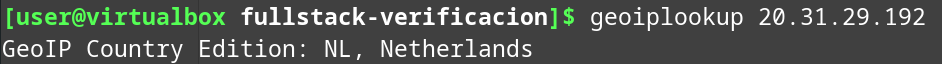
\includegraphics{../capturas/azure_geoip.png}
				} 
				\caption{Ubicación de los servidores}
			\end{subfigure}
			\linebreak
			
			\begin{subfigure}{\textwidth}
				\resizebox{\linewidth}{!}{%
					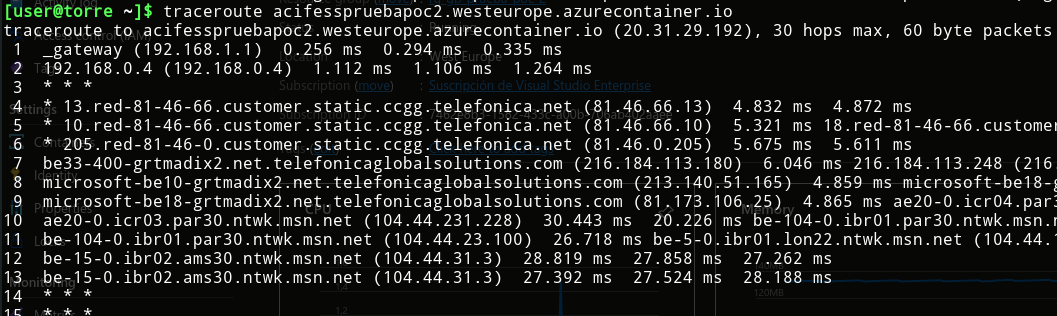
\includegraphics{../capturas/azure_traceroute3.png}
				} 
				\caption{\texttt{traceroute} contra el FQDN del frontend}
			\end{subfigure}

			
			\caption{Investigación de los detalles de la infraestructura (O. Salvador, 2022)}
		\end{figure}
	
	\bigskip
	\bigskip
	
	
	
	
	
	\subsection{Cuenta de almacenamiento}
	Este componente fue el primero que integré, en Noviemrbe. Originalmente había planeado usar un S3 en AWS, y tuve que rehacer las peticiones para adaptarlo. No hay un contenedor local con el que simular un Blob Storage como MinIO lo es para S3. En ambas plataformas subir y borrar imagenes de sus almacenamientos ha sido la parte mas difícil del desarrollo, pero AWS tenía mejor soporte y fue mas cómodo y rápido. Como expliqué en la sección \textit{Aplicación}, genero una URL con credenciales perecederos a la que subir la imagen. Cualquiera con esa URL puede subir una imagen, después de que se suba una los credenciales no tienen permiso para sobreescribirla. Durante el desarrollo tomaba las URL que genera el backend (no rellenaba a mano la URL que muestro) y probaba a subir imagenes manualmente, usando una vez más, cURL. 
	\linebreak
	
		\begin{figure}[htb]
			\centering
			\begin{subfigure}{\textwidth}
				\footnotesize
				\texttt{\$ curl -v -X PUT "https://<CUENTA\_DE\_ALMACENAMIENTO>.blob.core.windows.net/\\<CONTENEDOR\_DE\_ALMACENAMIENTO>/<NOMBRE\_DE\_IMAGEN>.png?<SHARED\_ACCESS\_SIGNATURE>"\ --data-binary @<IMAGEN\_A\_SUBIR>.png -H "x-ms-blob-type: BlockBlob"} 
			\end{subfigure}
			Comando para subir imagenes 
		\end{figure}

	\clearpage
	La depuración de la configuración de CORS (\textit{Cross-Origin Resource Sharing}) ha sido la parte más difícil del proyecto pese a su simpleza. Al principio no configuraba  \textit{Allowed} y \textit{Exposed headers}, que resultó ser la solución (\cite{cors_almacen}). Cuando no lo hacía y no funcionaba saque la conclusión erronea que se ve en las siguientes imágenes\footnote{Todas las imágenes están disponibles en el repositorio, en \texttt{documentacion/capturas}, para poderlas leer mejor. En particular, el apartado e), que he cortado para poderlo leer, es la imagen \texttt{azure\_cors\_firefox\_error.png}}, que se podía usar el FQDN sin protocolo ni puerto. Tambien muestran la dificultad de depurar, cuando todo parece estar en orden.
	\linebreak

		\begin{figure}[htb]
			\centering
			\begin{subfigure}{\textwidth}
				\centering
				\resizebox{.8\linewidth}{!}{%
					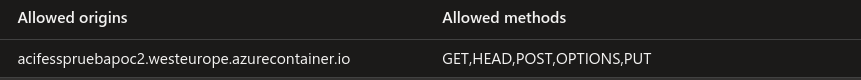
\includegraphics{../capturas/azure_cors_storage_account_config1.png}			
				}
				\resizebox{.8\linewidth}{!}{%
					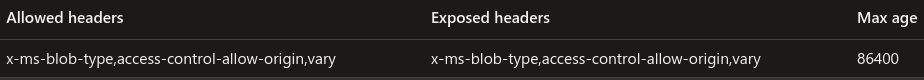
\includegraphics{../capturas/azure_cors_storage_account_config2.png}
				}
				\caption{Configuración de CORS de la cuenta de almacenamiento}
			\end{subfigure}
			\linebreak
			
			\begin{subfigure}{.92\linewidth}
				\inputminted[fontsize=\tiny, firstline=33, lastline=36, linenos, frame=single, breaklines]{javascript}{../../frontend/terraform/main.tf}
				\vspace{-.5cm}
				\caption{Carga de variables en Terraform, \texttt{main.tf}}
			\end{subfigure}
			\linebreak
			
			\begin{subfigure}{.36\textwidth}
				\inputminted[fontsize=\tiny, firstline=80, lastline=91, linenos, frame=single, breaklines]{javascript}{../../frontend/src/components/PostPrompt.tsx}
				\vspace{.8cm}
				\caption{Cabeceras, frontend, \texttt{PostPromt.tsx}}
			\end{subfigure}
			\begin{subfigure}{.55\textwidth}
				\centering
				\resizebox{\linewidth}{!}{%
					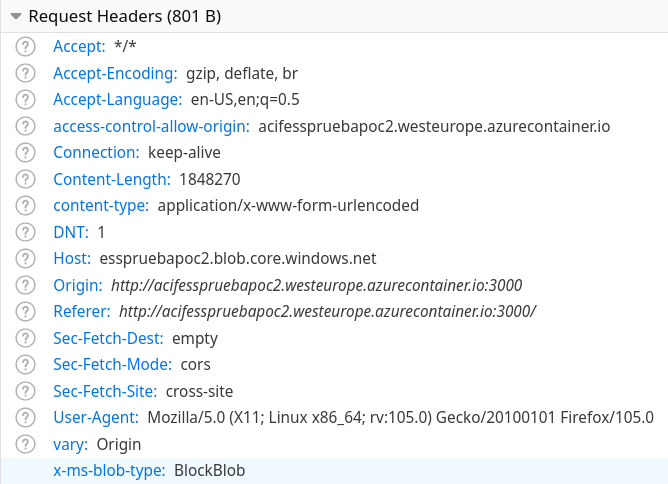
\includegraphics{../capturas/azure_cors_firefox_headers.png}
				}
				\caption{Cabeceras en la petición del navegador}
			\end{subfigure}
			\linebreak

			\begin{subfigure}{\textwidth}
				\centering
				\resizebox{\linewidth}{!}{%
					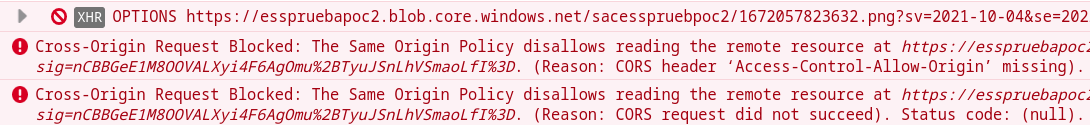
\includegraphics{../capturas/azure_cors_firefox_error2.png}
				}
				\caption{Fracaso de la petición PUT a la cuenta de almacenamiento desde el cliente}
			\end{subfigure}
			\caption{Depuración de CORS (O. Salvador, 2022)}
		\end{figure}














\clearpage
\section{Terraform}
Terraform es una herramienta puramente de aprovisionado de infraestructura. Permite contratarla y cambiarla, manteniendo control de versión. Desarrollado y mantenido por Hashicorp, fue publicado en 2014, bajo la licencia de código abierto Mozilla (MPLv2.0). 
\linebreak

Se basa en archivos con configuraciones para saber que desplegar. Pueden estar escritos en el ``Hashicorp Configuration Language'' (HCL) o en formato JSON. Estos contienen el estado \textit{deseado} de la infraestructura, los elementos que se quieren presentes (e implícitamente, los que no), y que propiedades deberían tener. Para ofrecer esta presentación uniforme de las configuraciones entre distintas plataformas, Terraform utiliza \textit{proveedores} que se encargan de los detalles del proceso de aprovisionado, abstrayéndolos del usuario.
\linebreak


Los elementos, \textit{bloques}, de un proyecto pueden tener uno de varios tipos, algunos de los principales son: declaraciones de variables, de proveedores, recursos, datos de recursos, y salidas. Para declarar variables (y opcionalmente darles un valor predeterminado) que usar en los demás bloques se usa \texttt{variable}. Con \texttt{required\_providers} y \texttt{provider} se especifica el proveedor y sus propiedades en el proyecto. El bloque principal es \texttt{resource}, donde se especifica un objeto que crear en en la plataforma destino. Los bloques \texttt{data} y \texttt{output} permiten recuperar información de la plataforma, detalles de objetos que ya estén creados \underline{durante} el proceso (para usar en otros bloques) y \underline{después} de la ejecución respectivamente (para usar en otros proyectos). Los bloques HCL deben seguir el siguiente formato:
\linebreak

	\begin{figure}[htb]
		\footnotesize
		\hspace{3.5cm}
		\texttt{<BLOCK TYPE>\ '<BLOCK LABEL>' '<BLOCK LABEL>' \{} 
		
		\hspace{4.5cm}
		\texttt{\color{gray}{\# Block body}}
		
		\hspace{4.5cm}
		\texttt{<IDENTIFIER>\ =\ <EXPRESSION>\ \color{gray}{\# Argument}} 

		\hspace{3.5cm}		
		\texttt{\}}
		\caption{Sintaxis de referencia, documentación de Hashicorp (\cite{hashicorp_lang1}, 2022)}
	\end{figure}
	

La extensión de la mayoría de archivos HCL en un proyecto de Terraform es \texttt{.tf}. En JSON los elementos siguen la misma estructura que en HCL, pero ligeramente adaptada y el prefijo de terraform antes de la extension (eg. \texttt{.tf.json}). Los nombres de los archivos es importante, en particular \texttt{variables.tf}, \texttt{providers.tf}, \texttt{main.tf}, y \texttt{outputs.tf}. Estos contienen los bloques antes mencionados, aunque, según la escala del proyecto pueden ir todos en el principal. Aparte de estos, hay otros archivos para el funcionamiento de Terraform que mencionaré en la siguiente sección, y \texttt{variables.tfvars}. En este no hay bloques, solo parejas de identificadores y expresiones (sus valores). Se puede usar para poblar las declaraciones de variables.






	\clearpage
	\subsection{Funcionamiento}
		Hashicorp ha hecho admirablemente sencillo la ``instalación'' de Terraform. Distribuyen un binario listo para usar, y trivialmente portable. En linux, con colocarlo en \texttt{/usr/local/bin} queda reconocido por la consola. Ofrece una miríada de opciones en su CLI. Los comandos principales son: \texttt{init}, \texttt{validate}, \texttt{plan}, \texttt{apply}, y \texttt{destroy}. 
		\linebreak
		
		El primer comando, \texttt{terraform init}: descarga los proveedores que se hayan indicado, crea algunos archivos para su operación y carga un estado remoto si se le indica. En Terraform el estado es una captura en local de los detalles de la implementación de la infraestructura como estaban en la plataforma objetivo la ultima vez que se actualizó. 
		\linebreak
		
		Este fichero es necesario para que Terraform funcione. ``El propósito principal del estado de Terraform es almacenar los enlaces entre los objetos en un sistema remoto y las instancias de recursos declarados en su configuración'' (\cite{hashicorp_state}). Se guardan los identificadores y propiedades de los recursos en el archivo \texttt{terraform.tfstate}, en formato JSON. Se pueden ver sus contenidos en cualquier momento con el comando \texttt{terraform show} Adicionalmente se genera una copia de seguridad, \texttt{terraform.tfstate.backup} automáticamente. A menudo contiene información comprometedora, como credenciales, es importante guardarlo de forma segura. 
		\linebreak
		
		Adicionalmente, el estado se puede guardar remotamente, para facilitar el desarrollo colaborativo y el uso en pipelines de CI/CD. Con el comando \texttt{terraform import} se puede crear o actualizar el estado del proyecto en la plataforma \textit{cloud} u \textit{on-prem}. Si el proyecto ya tiene los fuentes con los nombres de los recursos, también es capaz de poblarlos con su configuración en la plataforma (\cite{hashicorp_import}).
		\linebreak
		
		En el tercero, \texttt{terraform plan}, se convierten los archivos de configuraciones a un conjunto de pasos que Terraform puede seguir para alcanzar dicho estado deseado. Ejecutarlo automáticamente lanzará el segundo, \texttt{terraform validate}, que comprueba si los fuentes tienen una configuración valida. Si lo es, resuelve las variables. Recorre \texttt{variables.tf} y las puebla con \texttt{variables.tfvars}. Se puede especificar un fichero de variables con \texttt{-var-file variables.tfvars} Si hay mas en el \texttt{.tfvars} de las que se usan, Terraform avisará de ello. Si hay menos, y no tienen valor predeterminado son pedidas al usuario por TUI. El usuario puede sobreescribir las variables del fichero para una ejecucion de dos maneras. Puede incluir la opcion \texttt{-var nombre=``valor''} o exportar variables de sistema con el nombre de esta y el prefijo \texttt{TF\_VAR}. Por ejemplo, para la variable ``\texttt{rg\_name}'', exportar en la misma consola la variable ``\texttt{TF\_VAR\_rg\_name}''.
		\linebreak
		
		Lo siguiente que hace es recuperar el estado actual de cualquier objeto que ya este creado en la plataforma (\cite{hashicorp_plan}, \cite{hashicorp_plan_refresh}). Con la configuración previa actualizada, calcula las diferencias frente a la propuesta. El último paso para generar un plan es calcular un grafo de dependencias. Terraform hace esto recorriendose los fuentes, viendo los recursos mencionados, y añadiendo un nodo por cada uno. Las parejas de ``\texttt{<BLOCK LABEL>}'' indican dependencia del segundo al primero, los bloques que estén definidos dentro de otros a su padre, y los bloques que usen la etiqueta \texttt{depends\_on} al que mencionen (\cite{hashicorp_graph}). Después de añadir los nodos al grafo con las dependencias adecuadas, etiqueta a cada uno con meta-datos basándose en las diferencias entre el estado y la configuración, para saber que operaciones tomar con cada nodo. 
		\linebreak
		
		El grafo se puede generar independientemente con \texttt{terraform graph} en cualquier momento, solo para visualizar. El resultado del comando es el texto del grafo, en formato DOT. A continuación muestro un extracto del proyecto mas sencillo, el frontend (detalles en la siguiente sección), es solo una parte para no dedicarle una página\footnote{He generado los diagramas completos para todos los proyectos, y un \texttt{readme.md} con detalles de como generarlos. Están en la carpeta \texttt{documentacion/terraform-graph}}. 
		\linebreak
		
		\medskip
		
		\begin{figure}[htb]
			\centering
			\resizebox{.8\linewidth}{!}{%
				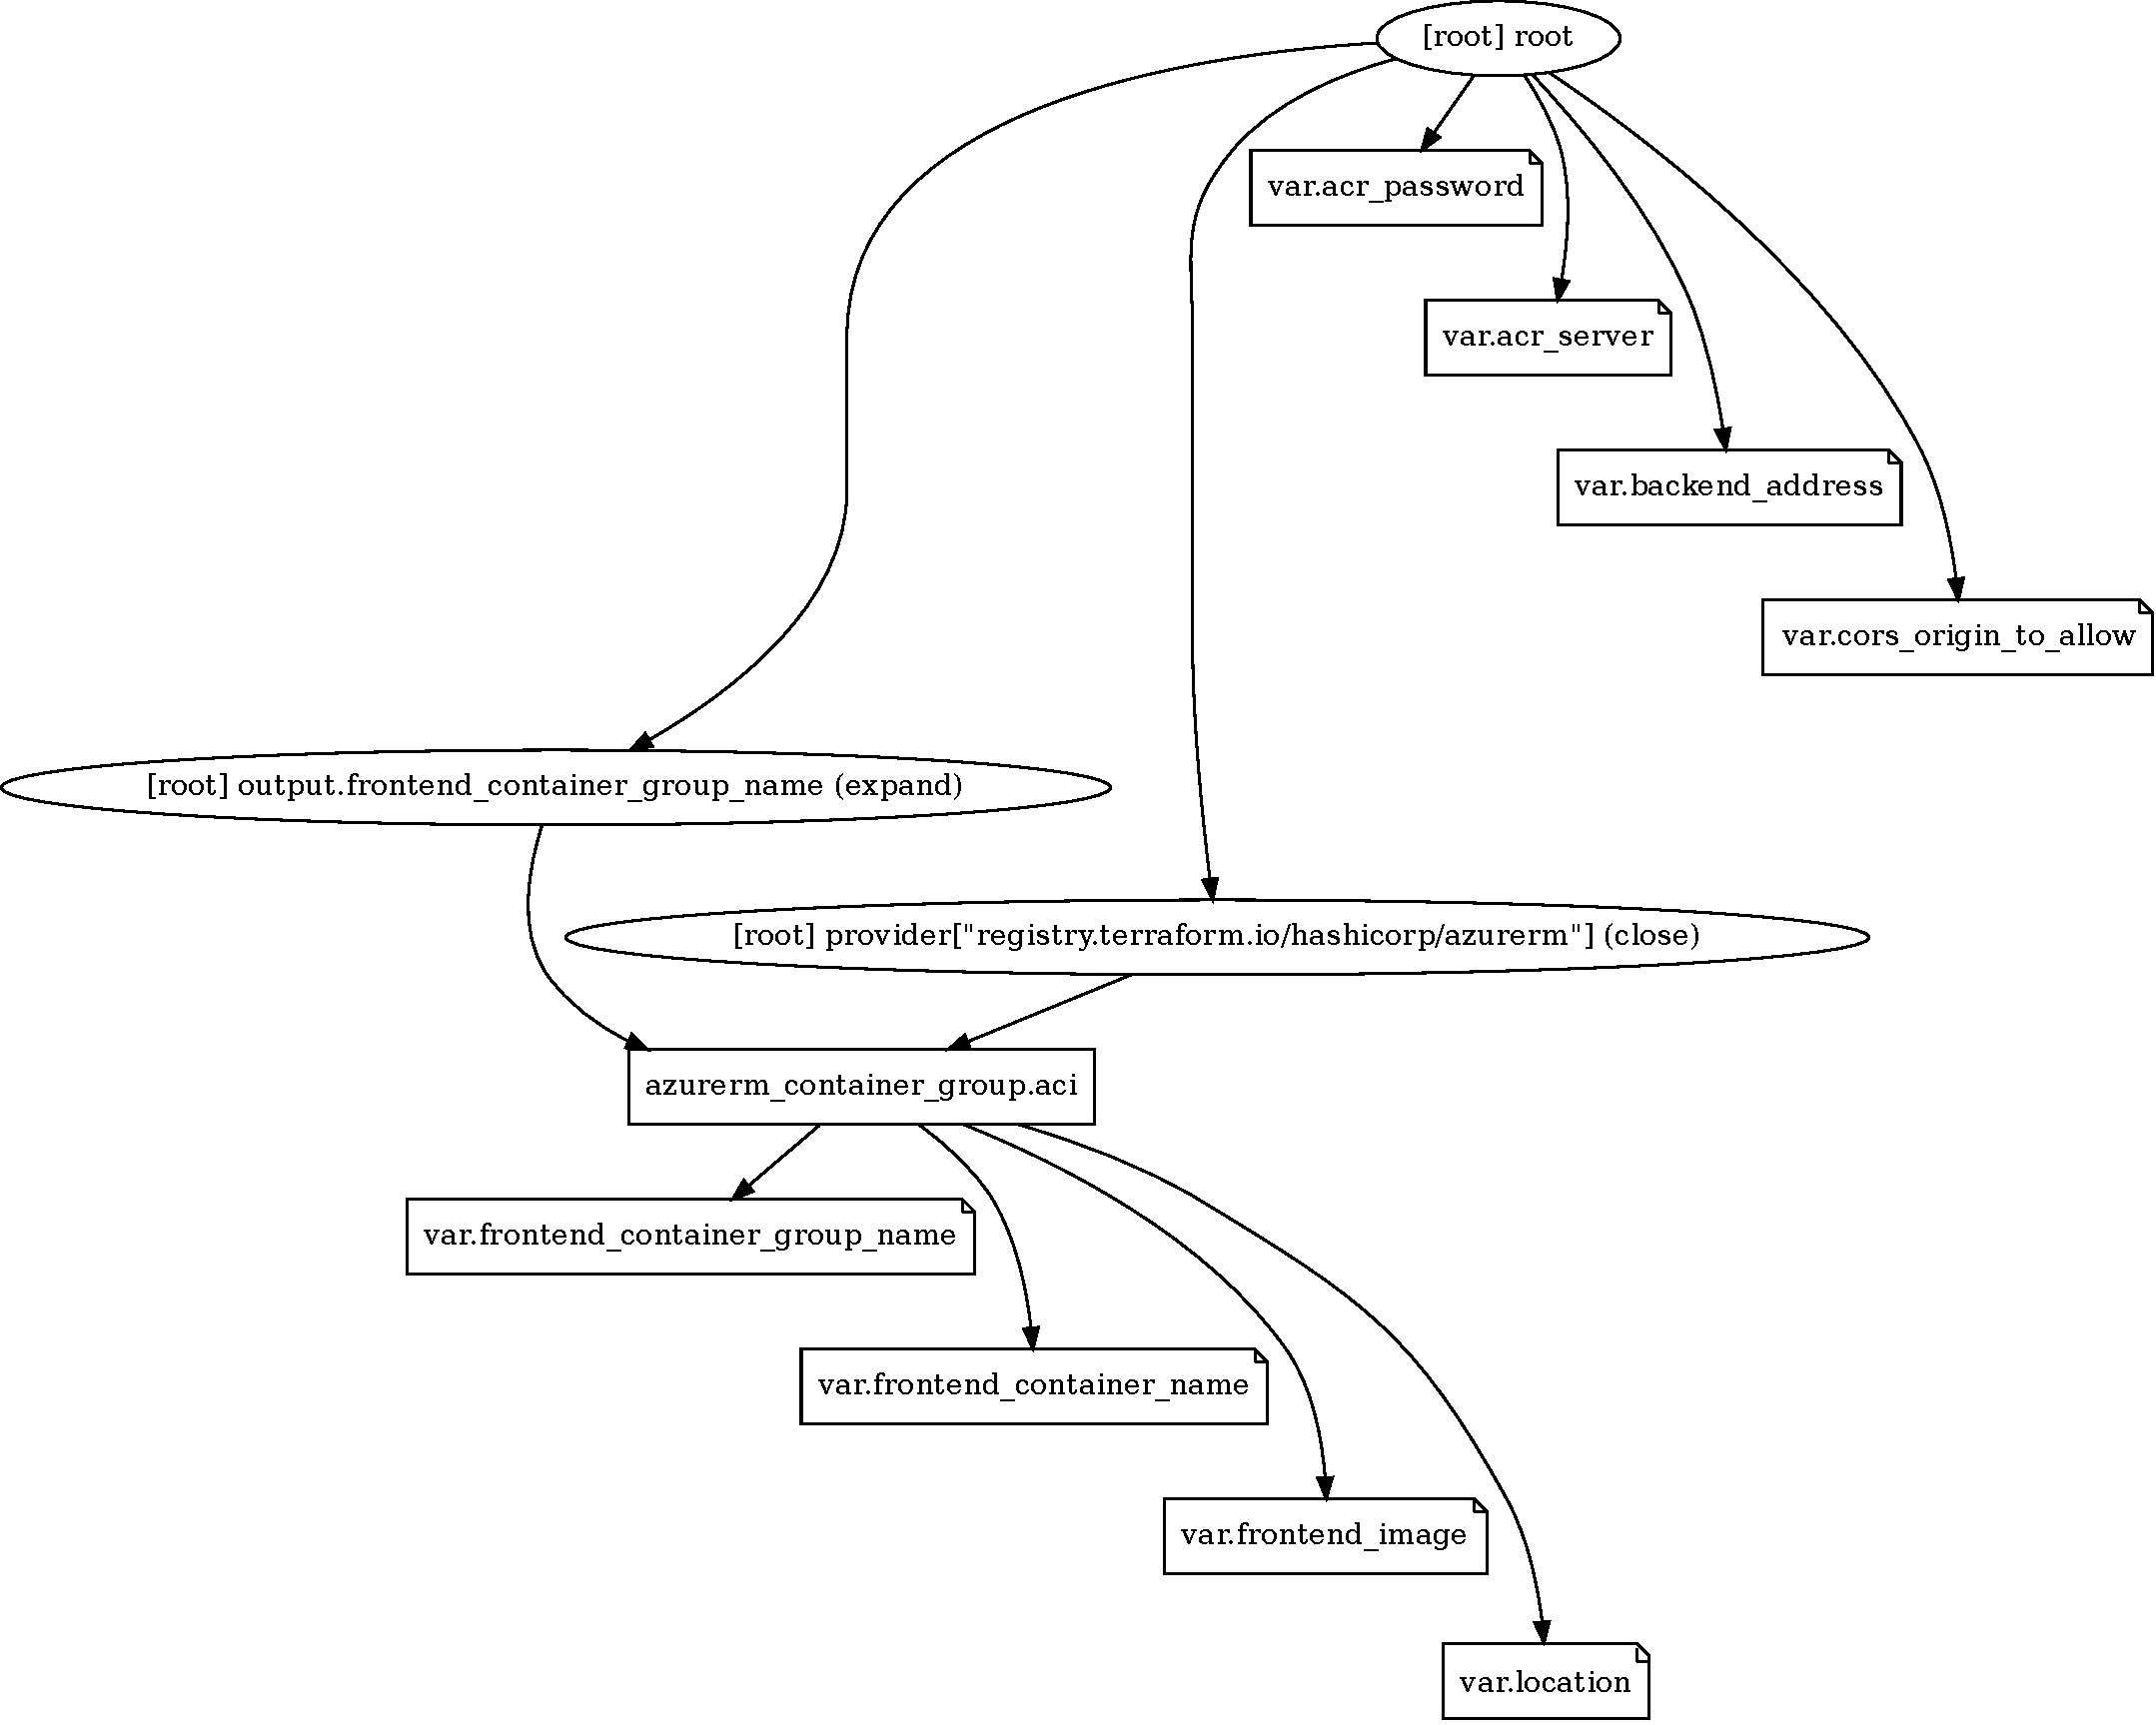
\includegraphics{../terraform-graph/demo-graph.pdf}
			}
			\caption{Extracto del grafo del frontend (O. Salvador, 2022)}
		\end{figure}
		
		\clearpage
		
		Finalmente, Terraform calcula y muestra la serie de pasos que Terraform seguirá para alcanzar el estado deseado, si hay diferencias. Los cambios a la infraestructura propuestos pueden ser: crear nuevos recursos, destruir recursos existentes, y actualizar un recurso existente, que a veces requiere la destrucción y sustitución (\textit{creación in-place}) del recurso.
		\linebreak
		
			\begin{figure}[htb]
				\begin{subfigure}{.49\textwidth}
					\centering
					\resizebox{.8\linewidth}{!}{%
						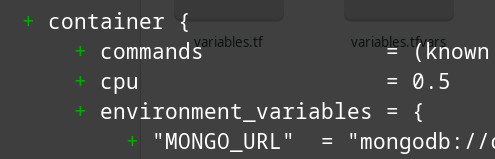
\includegraphics{../capturas/azure_terraform_create.png}
					}
					\caption{Creación}
				\end{subfigure}
				\begin{subfigure}{.49\textwidth}
					\centering
					\resizebox{\linewidth}{!}{%
						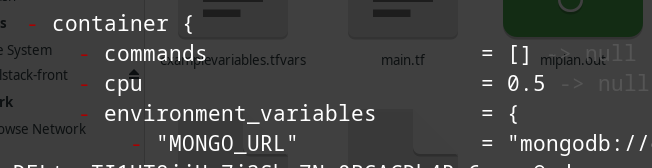
\includegraphics{../capturas/azure_terraform_destroy.png}
					}
					\caption{Destrucción}
				\end{subfigure}
				\linebreak
				
				\begin{subfigure}{.8\textwidth}
					\resizebox{\linewidth}{!}{%
						\vspace{1cm}
						\hspace{2.2cm}
						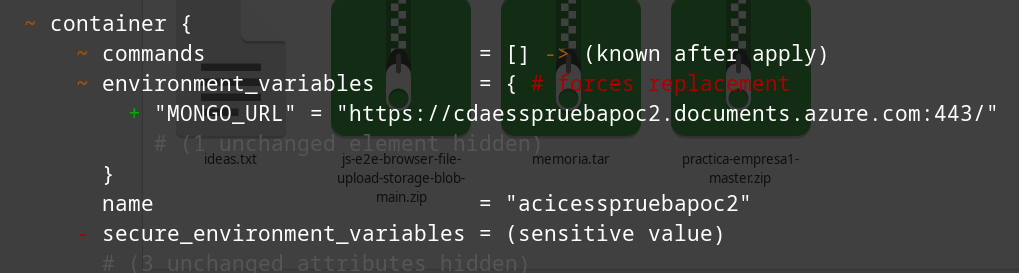
\includegraphics{../capturas/azure_terraform_replace.png}
					}
					\caption{Reemplazo}
				\end{subfigure}
				\caption{Planificación de operaciones contra la plataforma (O. Salvador, 2022)}
			\end{figure}

		La ejecución de la planificación sin más opciones genera un \textit{plan especulativo}, \underline{solo} en memoria y sin intención de ser aplicado. Este puede ser usado para comprobar si los efectos son los deseados. Para guardarlo es necesario añadir la opción \texttt{-out=FICHERO\_DESTINO.out} (\cite{hashicorp_plan}).
		\linebreak
		
		El penúltimo comando mencionado es \texttt{terraform apply}. Implícitamente desata una planificación, con los pasos antes descritos, incluida la importación del estado actual en la plataforma. Alternativamente se le puede alimentar un plan ya calculado incluyendo su nombre (eg. \texttt{terraform apply FICHERO\_DESTINO.out} para el plan anterior), al haber resuelto las variables para este, no es necesario volverlo a hacer. Terraform utiliza el grafo de nodos para crear los recursos. Lo usa para encontrar nodos sin dependencias, y poder paralelizar sus operaciones. Por defecto busca un paralelismo de diez recursos.
		\linebreak
		
		Para quitar los recursos propuestos en los fuentes de configuración de la plataforma, y dejarla yerma Terraform ofrece dos opciones. El último comando que he presentado es \texttt{terraform destroy}. La otra opción es realizar un nuevo \texttt{terraform apply}, añadiendo la opción \texttt{-destroy}. En ambos el resultado es el mismo, Terraform recorrerá el grafo de dependencias eliminando todos los nodos. Si es posible, paralelizará las operaciones.
		\linebreak
		
		
		% ---
		
		Durante todos los comandos y sus pasos Terraform necesita interactuar con la plataforma objetivo. Lo consigue a través de proveedores. Estos son \textit{plug-ins}, componentes adicionales que añaden la funcionalidad especifica para su plataforma particular. Esta no tiene que ser en la nube, hay proveedores para aprovisionado en plataformas \textit{on-prem}: \cite{onprem_provider1}, \cite{onprem_provider2}, \cite{onprem_provider3}. Permiten separar el desarrollo de proyectos Terraform con configuraciones a alto nivel, uniforme entre plataformas, y los detalles específicos de la implementación de su API correspondiente.
		\linebreak
		
		Según Hashicorp, ``Las principales responsabilidades de los Plugins Proveedores son:
			\begin{itemize}
				%\addtolength{\itemindent}{0.80cm}
				\itemsep0em 
				\item Inicialización de cualquier biblioteca incluida que se utilice para realizar llamadas a la API.
				\item Autenticación con el proveedor de infraestructura
				\item Definir los recursos que se asignan a servicios específicos
			\end{itemize}
		'' (\cite{hashicorp_plugins} § Terraform Plugins)
		\linebreak
		
		
		El binario principal, \textit{Terraform Core} no incluye proveedores. En su lugar, cuando se ejecuta \texttt{terraform init} busca en los archivos de configuraciones del proyecto y descarga del \textit{Terraform Registry} los proveedores que encuentre declarados. No son necesarios mas pasos.
		\linebreak
		
		\begin{figure}[htb]
			\centering
			\begin{subfigure}{.35\linewidth}
				\inputminted[fontsize=\scriptsize, firstline=1, lastline=8, linenos, frame=single, breaklines]{javascript}{../../terraform/providers.tf}
				\caption{Declaración}
			\end{subfigure}
			\hspace{1.5cm}
			\begin{subfigure}{.4\linewidth}
				\inputminted[fontsize=\scriptsize, firstline=10, lastline=15, linenos, frame=single, breaklines]{javascript}{../../terraform/providers.tf}
				\vspace{.99cm}
				\caption{Configuración}
			\end{subfigure}
			\caption{Declaración y configuración del proveedor, \texttt{providers.tf} (O. Salvador, 2022)}
		\end{figure}
		
		En el \textit{Registry} hay más de mil proveedores hechos por Hashicorp y por la comunidad, señalados como tal. También contiene \textit{módulos}, pequeños proyectos, configuraciones que permiten trabajar con conjuntos de recursos como uno solo. Un usuario de Terraform puede usarlos, ya que son publicamente accesibles, o crear los suyos propios.	Crear módulos propios fomenta el código reutilizable, y en un proyecto mayor, o para una organización tener estas plantillas facilita el desarrollo. Para las necesidades de este proyecto he considerado que superaban su ámbito.






	\clearpage
	\subsection{Implementación}
		He explicado el funcionamiento general de Terraform, ahora detallaré como lo he usado yo para generar la infraestructura necesaria para este proyecto. He diseñado la infraestructura al mismo tiempo que aprendía como montarla en Terraform, por el beneficio de poderla eliminar y montar a menudo, reduciendome el coste. Lo reflejaré en esta sección, explicando varios pasos en falso que tomé.
	 \linebreak
	 
	 Como mencioné en la sección \textit{Infraestructura e integración}, el frontend necesita al backend antes de crearse, y este a los demás componentes. Para solucionar esto, he dividido la infraestructura en tres proyectos de Terraform. Un primer proyecto \texttt{/terraform} monta todo salvo los grupos de contenedores. Después es necesario entrar a la carpetas \texttt{/backend/terraform} y \texttt{/frontend/terraform} y aplicarlos, en ese orden. Estos dos necesitan encontrar las imágenes Docker con su código en el ACR. He conseguido una implementación en la que los proyectos sucesivos recuperan por su cuenta los valores que necesitan de los recursos generados en sus predecesores.
	 \linebreak
	 
	\begin{figure}[htb]
		\centering
		\resizebox{\linewidth}{!}{%
			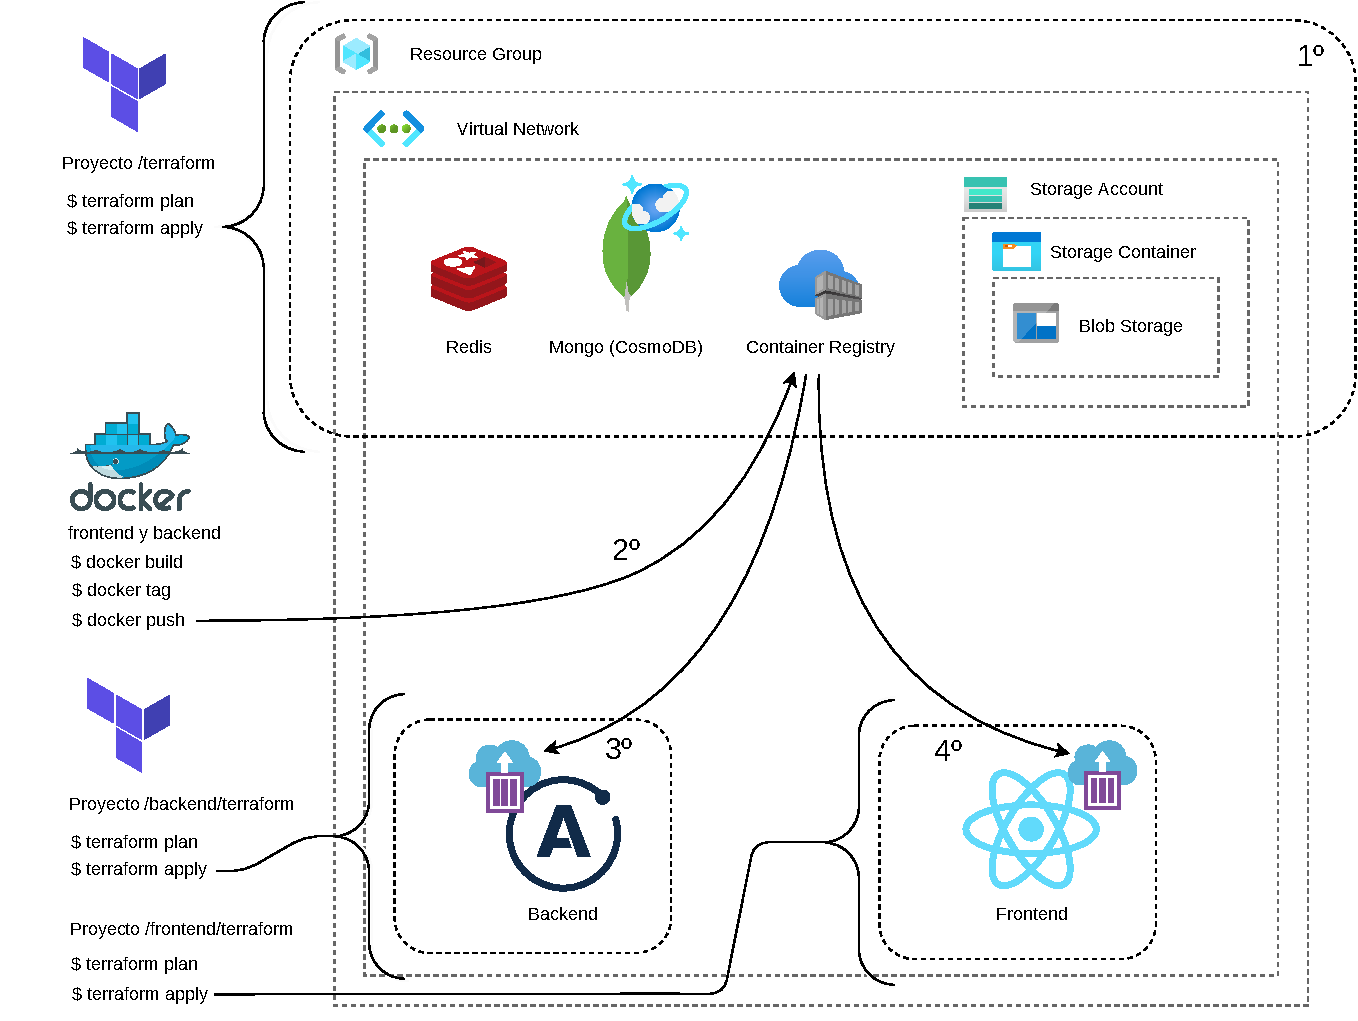
\includegraphics{../drawio/terraform-etapas.drawio.pdf}
		}
		\caption{Tres proyectos de Terraform y dos imagenes de Docker (O. Salvador, 2022)}
	\end{figure}
	
	\clearpage
	Terraform es capaz de encontrar los recursos porque tiene sus nombres y porque uso bloques \textit{data}. Para que tenga los nombres es necesario declararlos en el \texttt{variables.tfvars} de cada proyecto. Podría usar un único archivo para los tres, pero como expliqué en la subsección anterior, causaría avisos, ya que Terraform vería que hay variables en el archivo que no son usadas por el proyecto. Dado que solo es necesario escribir los nombres de los recursos que buscar, se pueden llenar los tres \texttt{.tfvars} a priori. 
	\linebreak
	
	En el siguiente extracto utilizo la variable con el nombre y grupo de recursos de la cuenta de almacenamiento para identificarla. Con esos dos datos, Terraform entiende que tiene que buscar el recurso y resolver sus detalles al llamarlo por su pareja de etiquetas. Las dos etiquetas de un bloque detrás del tipo de bloque, son el tipo de recurso dentro del proveedor, y el nombre por el que identificar el recurso durante el \texttt{plan} y \texttt{apply} (en el grafo de dependencias) del proyecto. Al juntar estas dos, se identifica al recurso inequivocamente y se pueden acceder a sus propiedades. En el caso de la cuenta de almacenamiento, el backend necesita ser alimentado su nombre, el nombre del contenedor de almacenamiento que he creado en el primer proyecto, y la llave de administración. Las dos primeras se saben antes de montar la infraestructura, pero la llave se genera aleatoriamente con cada despliegue del proyecto. Usar el bloque data y referirme a sus contenidos como muestro ahorra ahorra al usuario actualizarlo su valor de manera manual.
	\linebreak
	
		\begin{figure}[htb]
			\centering
			\begin{subfigure}{0.7\textwidth}
				\inputminted[fontsize=\scriptsize, firstline=6, lastline=9, linenos, frame=single, breaklines]{dockerfile}{../../backend/terraform/main.tf}
				\inputminted[fontsize=\scriptsize, firstline=21, lastline=21, linenos, frame=single, breaklines]{dockerfile}{../../backend/terraform/main.tf}
				\inputminted[fontsize=\scriptsize, firstline=45, lastline=45, linenos, frame=single, breaklines]{dockerfile}{../../backend/terraform/main.tf}
				\inputminted[fontsize=\scriptsize, firstline=51, lastline=51, linenos, frame=single, breaklines]{dockerfile}{../../backend/terraform/main.tf}
				\inputminted[fontsize=\scriptsize, firstline=56, lastline=59, linenos, frame=single, breaklines]{dockerfile}{../../backend/terraform/main.tf}
			\end{subfigure}
			\caption{Uso de bloques \textit{data} para las variables de entorno de los contenedores (O. Salvador, 2022)}
		\end{figure}
	
	Terraform usa el proveedor para recuperar la información de recursos que se han creado en proyectos anteriores (y que por tanto no estan disponibles por parejas de etiquetas) usando el API de la plataforma. Luego alimento los detalles que necesito de estos recursos a los contendores, y el código en ellos se los encuentra como variables de entorno, completamente abstraído de como ha llegado hasta ahí. Es de esta manera que puedo pasar las variables de entorno que piden en su código a los contenedores del backend (connection string de Mongo; dirección y credenciales de Redis; y credenciales de la cuenta de almacenamiento) y frontend (dirección del backend), actualizandolas automáticamente.
	\linebreak
	
	La etiqueta de tipo de recurso del proveedor normalmente le sirve a este para inferir las dependencias con los demás recursos. Sin embargo, durante mi desarrollo tuve una ocasión en la que falló. 
		% hablar de cors, que ahora es seguro y solo se conecta frontend
		% hablar de whitelisted_ip, aunque ahora este comentado

	He encontrado dos \textit{issues} cerrados (\cite{tf_depends3}, \cite{tf_depends2}) y uno abierto (\cite{tf_depends1}) con problemas similares. En mi caso lo soluciono depends on
	

	
	
	
\clearpage
\section{Ansible}
tbc

\section{Comparación}
tbc dsaa\cite{rediscode}aa\cite{knuth-fa}

% moverlo a comparacion
%\subsection{Contexto} % a lo mejor moverlo a lecciones aprendidas? segun espacio, hacer seccion infraestructura como codigo, y meter tf y ans dentro
%otras herramientas, imperativas

\section{Conclusión}
tbc

\section{Lecciones aprendidas}

a



\end{flushleft}

\printbibliography

\end{document}
